\documentclass[twoside]{book}

% Packages required by doxygen
\usepackage{fixltx2e}
\usepackage{calc}
\usepackage{doxygen}
\usepackage[export]{adjustbox} % also loads graphicx
\usepackage{graphicx}
\usepackage[utf8]{inputenc}
\usepackage{makeidx}
\usepackage{multicol}
\usepackage{multirow}
\PassOptionsToPackage{warn}{textcomp}
\usepackage{textcomp}
\usepackage[nointegrals]{wasysym}
\usepackage[table]{xcolor}

% Font selection
\usepackage[T1]{fontenc}
\usepackage[scaled=.90]{helvet}
\usepackage{courier}
\usepackage{amssymb}
\usepackage{sectsty}
\renewcommand{\familydefault}{\sfdefault}
\allsectionsfont{%
  \fontseries{bc}\selectfont%
  \color{darkgray}%
}
\renewcommand{\DoxyLabelFont}{%
  \fontseries{bc}\selectfont%
  \color{darkgray}%
}
\newcommand{\+}{\discretionary{\mbox{\scriptsize$\hookleftarrow$}}{}{}}

% Page & text layout
\usepackage{geometry}
\geometry{%
  a4paper,%
  top=2.5cm,%
  bottom=2.5cm,%
  left=2.5cm,%
  right=2.5cm%
}
\tolerance=750
\hfuzz=15pt
\hbadness=750
\setlength{\emergencystretch}{15pt}
\setlength{\parindent}{0cm}
\setlength{\parskip}{3ex plus 2ex minus 2ex}
\makeatletter
\renewcommand{\paragraph}{%
  \@startsection{paragraph}{4}{0ex}{-1.0ex}{1.0ex}{%
    \normalfont\normalsize\bfseries\SS@parafont%
  }%
}
\renewcommand{\subparagraph}{%
  \@startsection{subparagraph}{5}{0ex}{-1.0ex}{1.0ex}{%
    \normalfont\normalsize\bfseries\SS@subparafont%
  }%
}
\makeatother

% Headers & footers
\usepackage{fancyhdr}
\pagestyle{fancyplain}
\fancyhead[LE]{\fancyplain{}{\bfseries\thepage}}
\fancyhead[CE]{\fancyplain{}{}}
\fancyhead[RE]{\fancyplain{}{\bfseries\leftmark}}
\fancyhead[LO]{\fancyplain{}{\bfseries\rightmark}}
\fancyhead[CO]{\fancyplain{}{}}
\fancyhead[RO]{\fancyplain{}{\bfseries\thepage}}
\fancyfoot[LE]{\fancyplain{}{}}
\fancyfoot[CE]{\fancyplain{}{}}
\fancyfoot[RE]{\fancyplain{}{\bfseries\scriptsize Generated by Doxygen }}
\fancyfoot[LO]{\fancyplain{}{\bfseries\scriptsize Generated by Doxygen }}
\fancyfoot[CO]{\fancyplain{}{}}
\fancyfoot[RO]{\fancyplain{}{}}
\renewcommand{\footrulewidth}{0.4pt}
\renewcommand{\chaptermark}[1]{%
  \markboth{#1}{}%
}
\renewcommand{\sectionmark}[1]{%
  \markright{\thesection\ #1}%
}

% Indices & bibliography
\usepackage{natbib}
\usepackage[titles]{tocloft}
\setcounter{tocdepth}{3}
\setcounter{secnumdepth}{5}
\makeindex

% Hyperlinks (required, but should be loaded last)
\usepackage{ifpdf}
\ifpdf
  \usepackage[pdftex,pagebackref=true]{hyperref}
\else
  \usepackage[ps2pdf,pagebackref=true]{hyperref}
\fi
\hypersetup{%
  colorlinks=true,%
  linkcolor=blue,%
  citecolor=blue,%
  unicode%
}

% Custom commands
\newcommand{\clearemptydoublepage}{%
  \newpage{\pagestyle{empty}\cleardoublepage}%
}

\usepackage{caption}
\captionsetup{labelsep=space,justification=centering,font={bf},singlelinecheck=off,skip=4pt,position=top}

%===== C O N T E N T S =====

\begin{document}

% Titlepage & ToC
\hypersetup{pageanchor=false,
             bookmarksnumbered=true,
             pdfencoding=unicode
            }
\pagenumbering{alph}
\begin{titlepage}
\vspace*{7cm}
\begin{center}%
{\Large My Project }\\
\vspace*{1cm}
{\large Generated by Doxygen 1.8.13}\\
\end{center}
\end{titlepage}
\clearemptydoublepage
\pagenumbering{roman}
\tableofcontents
\clearemptydoublepage
\pagenumbering{arabic}
\hypersetup{pageanchor=true}

%--- Begin generated contents ---
\chapter{online-\/bookstore}
\label{md_README}
\Hypertarget{md_README}
\input{md_README}
\chapter{Hierarchical Index}
\section{Class Hierarchy}
This inheritance list is sorted roughly, but not completely, alphabetically\+:\begin{DoxyCompactList}
\item \contentsline{section}{Customer}{\pageref{classCustomer}}{}
\item \contentsline{section}{Menu}{\pageref{classMenu}}{}
\begin{DoxyCompactList}
\item \contentsline{section}{Customer\+Menu}{\pageref{classCustomerMenu}}{}
\item \contentsline{section}{Main\+Menu}{\pageref{classMainMenu}}{}
\item \contentsline{section}{Product\+Menu}{\pageref{classProductMenu}}{}
\item \contentsline{section}{Shopping\+Menu}{\pageref{classShoppingMenu}}{}
\end{DoxyCompactList}
\item \contentsline{section}{Payment}{\pageref{classPayment}}{}
\begin{DoxyCompactList}
\item \contentsline{section}{Cash}{\pageref{classCash}}{}
\item \contentsline{section}{Check}{\pageref{classCheck}}{}
\item \contentsline{section}{Credit\+Card}{\pageref{classCreditCard}}{}
\end{DoxyCompactList}
\item \contentsline{section}{Product}{\pageref{classProduct}}{}
\begin{DoxyCompactList}
\item \contentsline{section}{Book}{\pageref{classBook}}{}
\item \contentsline{section}{Magazine}{\pageref{classMagazine}}{}
\item \contentsline{section}{Music\+CD}{\pageref{classMusicCD}}{}
\end{DoxyCompactList}
\item \contentsline{section}{Product\+To\+Purchase}{\pageref{classProductToPurchase}}{}
\item \contentsline{section}{Shopping\+Cart}{\pageref{classShoppingCart}}{}
\end{DoxyCompactList}

\chapter{Class Index}
\section{Class List}
Here are the classes, structs, unions and interfaces with brief descriptions\+:\begin{DoxyCompactList}
\item\contentsline{section}{\hyperlink{classBook}{Book} }{\pageref{classBook}}{}
\item\contentsline{section}{\hyperlink{classCash}{Cash} }{\pageref{classCash}}{}
\item\contentsline{section}{\hyperlink{classCheck}{Check} }{\pageref{classCheck}}{}
\item\contentsline{section}{\hyperlink{classCreditCard}{Credit\+Card} }{\pageref{classCreditCard}}{}
\item\contentsline{section}{\hyperlink{classCustomer}{Customer} \\*\hyperlink{classCustomer}{Customer} class }{\pageref{classCustomer}}{}
\item\contentsline{section}{\hyperlink{classCustomerMenu}{Customer\+Menu} \\*\hyperlink{classCustomerMenu}{Customer\+Menu} class }{\pageref{classCustomerMenu}}{}
\item\contentsline{section}{\hyperlink{classMagazine}{Magazine} \\*\hyperlink{classMagazine}{Magazine} class inherits from product class }{\pageref{classMagazine}}{}
\item\contentsline{section}{\hyperlink{classMainMenu}{Main\+Menu} \\*\hyperlink{classMainMenu}{Main\+Menu} class }{\pageref{classMainMenu}}{}
\item\contentsline{section}{\hyperlink{classMenu}{Menu} \\*\hyperlink{classMenu}{Menu} class }{\pageref{classMenu}}{}
\item\contentsline{section}{\hyperlink{classMusicCD}{Music\+CD} \\*\hyperlink{classMusicCD}{Music\+CD} class inherits from product class }{\pageref{classMusicCD}}{}
\item\contentsline{section}{\hyperlink{classPayment}{Payment} \\*\hyperlink{classPayment}{Payment} class }{\pageref{classPayment}}{}
\item\contentsline{section}{\hyperlink{classProduct}{Product} \\*\hyperlink{classProduct}{Product} class }{\pageref{classProduct}}{}
\item\contentsline{section}{\hyperlink{classProductMenu}{Product\+Menu} }{\pageref{classProductMenu}}{}
\item\contentsline{section}{\hyperlink{classProductToPurchase}{Product\+To\+Purchase} }{\pageref{classProductToPurchase}}{}
\item\contentsline{section}{\hyperlink{classShoppingCart}{Shopping\+Cart} }{\pageref{classShoppingCart}}{}
\item\contentsline{section}{\hyperlink{classShoppingMenu}{Shopping\+Menu} }{\pageref{classShoppingMenu}}{}
\end{DoxyCompactList}

\chapter{Class Documentation}
\hypertarget{classBook}{}\section{Book Class Reference}
\label{classBook}\index{Book@{Book}}
Inheritance diagram for Book\+:\begin{figure}[H]
\begin{center}
\leavevmode
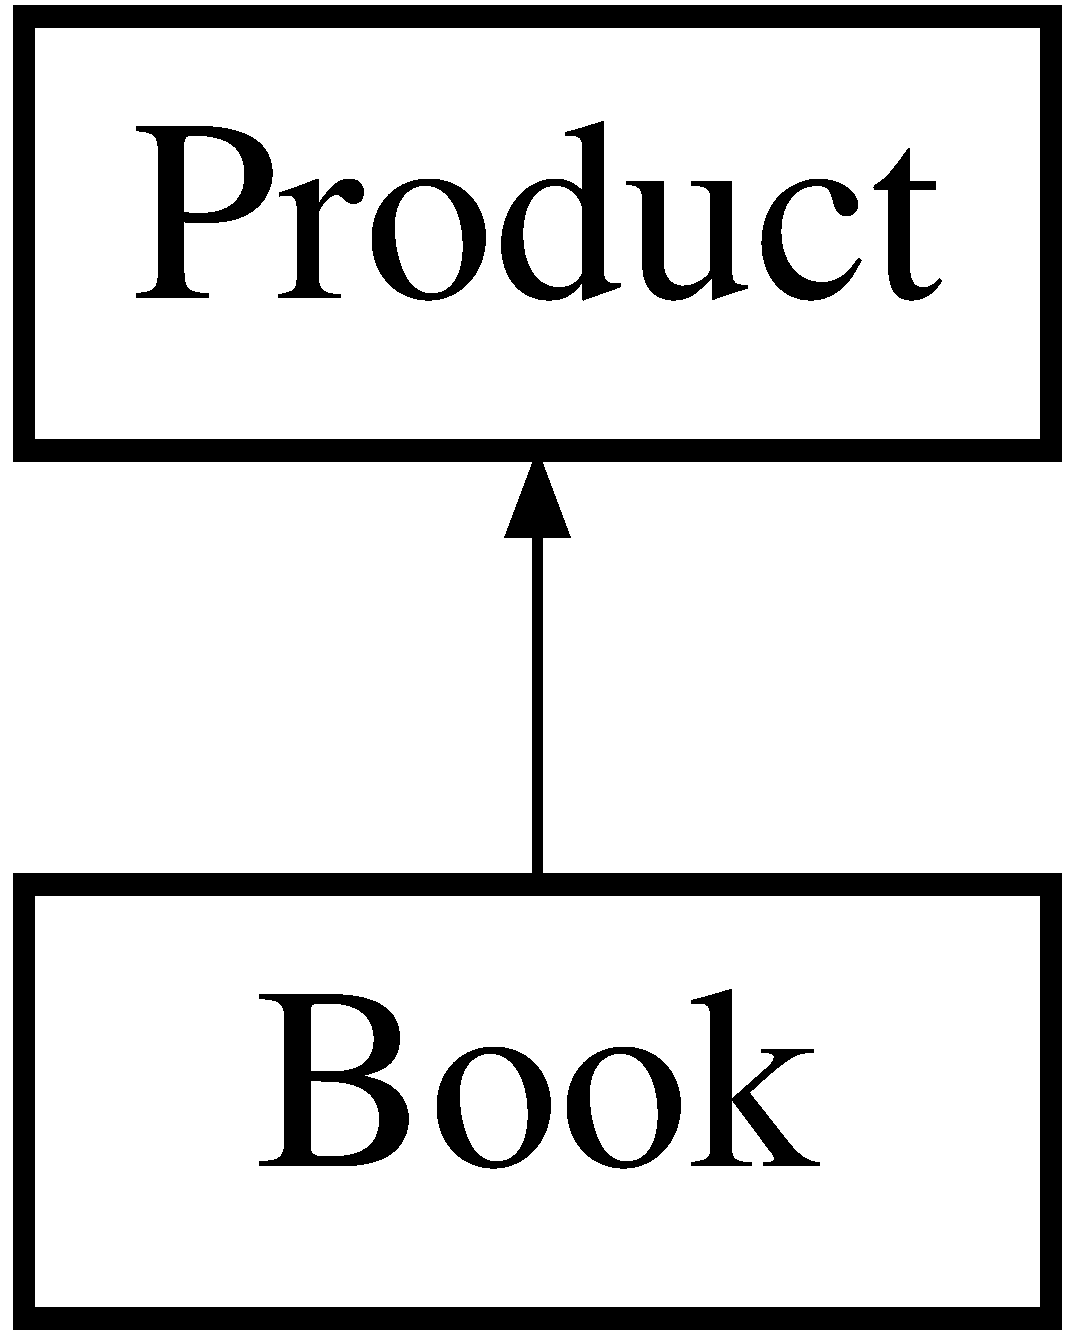
\includegraphics[height=2.000000cm]{classBook}
\end{center}
\end{figure}
\subsection*{Public Member Functions}
\begin{DoxyCompactItemize}
\item 
\mbox{\Hypertarget{classBook_af4bdcf29993e54f93e83af0f70648aac}\label{classBook_af4bdcf29993e54f93e83af0f70648aac}} 
{\bfseries Book} (int, string, double, string, string, int)
\item 
\mbox{\Hypertarget{classBook_aea2d37325e0b9f93637e3a47d8e2855b}\label{classBook_aea2d37325e0b9f93637e3a47d8e2855b}} 
{\bfseries Book} (int, string, double)
\item 
\mbox{\Hypertarget{classBook_ab430d9632f670b298b19c7b3e8d9acfc}\label{classBook_ab430d9632f670b298b19c7b3e8d9acfc}} 
void {\bfseries print\+Properties} ()
\item 
\mbox{\Hypertarget{classBook_a357d171d5d7c90340ee91a137edf958f}\label{classBook_a357d171d5d7c90340ee91a137edf958f}} 
string {\bfseries get\+Author} () const
\item 
\mbox{\Hypertarget{classBook_a837c5dbedad676a780b955c7ccfba859}\label{classBook_a837c5dbedad676a780b955c7ccfba859}} 
void {\bfseries set\+Author} (string)
\item 
\mbox{\Hypertarget{classBook_ad96401e4cfcc4adb2205a1a8ddbaa7e8}\label{classBook_ad96401e4cfcc4adb2205a1a8ddbaa7e8}} 
string {\bfseries get\+Publisher} () const
\item 
\mbox{\Hypertarget{classBook_ae1cc54edd9af29d7f05ef56a3a3039fc}\label{classBook_ae1cc54edd9af29d7f05ef56a3a3039fc}} 
void {\bfseries set\+Publisher} (string)
\item 
\mbox{\Hypertarget{classBook_a3199f3761e7b6a56af066028cd238d3b}\label{classBook_a3199f3761e7b6a56af066028cd238d3b}} 
int {\bfseries get\+Page} () const
\item 
\mbox{\Hypertarget{classBook_aa816ee3806073b0600aeb6d0f92cebfc}\label{classBook_aa816ee3806073b0600aeb6d0f92cebfc}} 
void {\bfseries set\+Page} (int)
\end{DoxyCompactItemize}


The documentation for this class was generated from the following files\+:\begin{DoxyCompactItemize}
\item 
Book.\+h\item 
Book.\+cpp\end{DoxyCompactItemize}

\hypertarget{classCash}{}\section{Cash Class Reference}
\label{classCash}\index{Cash@{Cash}}
Inheritance diagram for Cash\+:\begin{figure}[H]
\begin{center}
\leavevmode
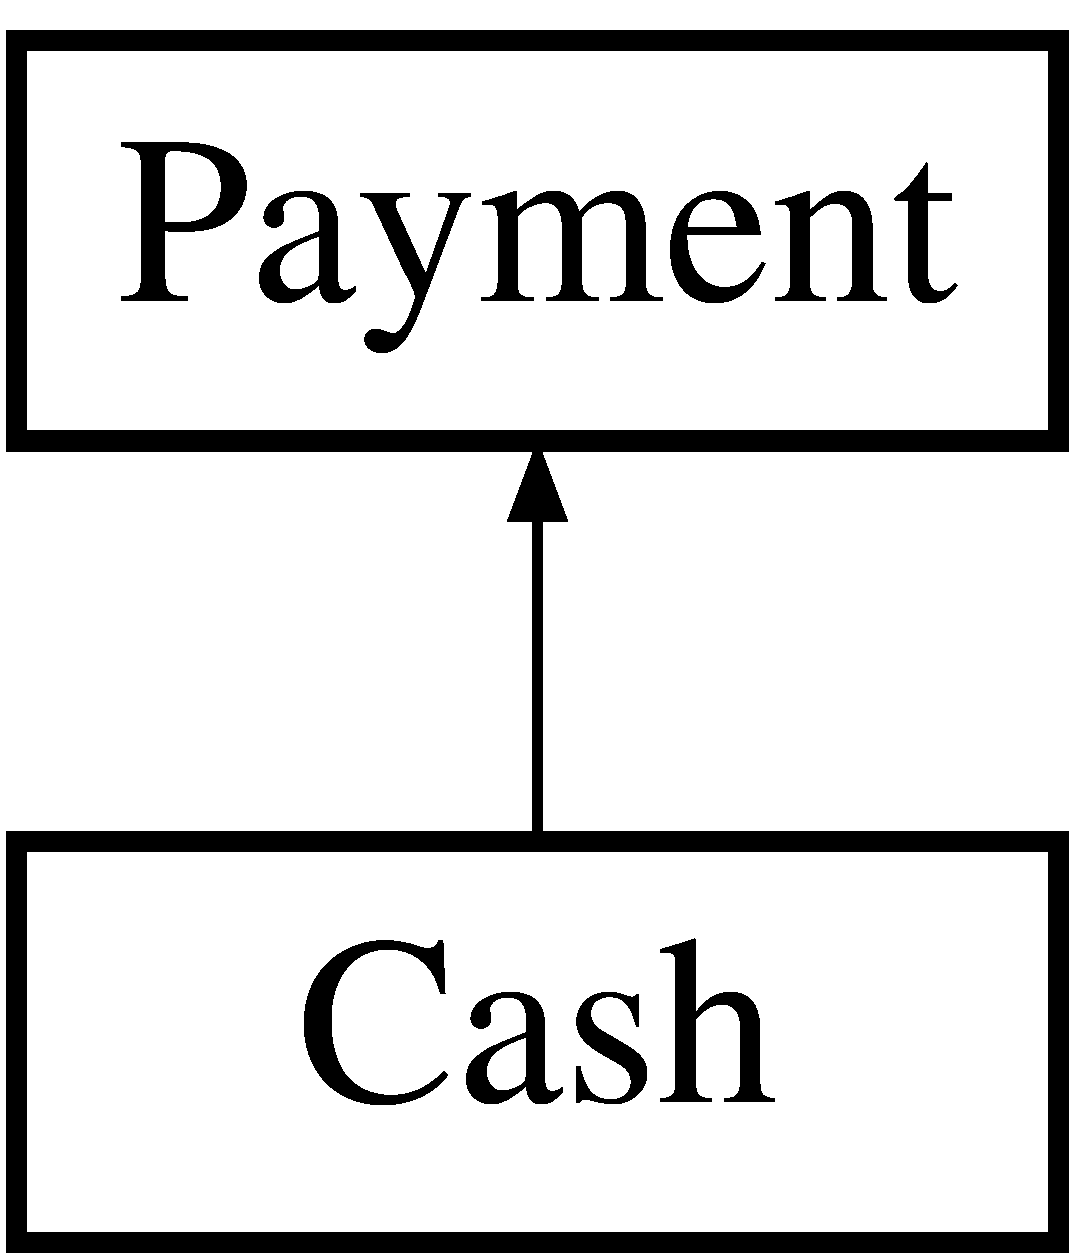
\includegraphics[height=2.000000cm]{classCash}
\end{center}
\end{figure}
\subsection*{Public Member Functions}
\begin{DoxyCompactItemize}
\item 
\mbox{\Hypertarget{classCash_a60e367204f5992a0a954933039ce0ff5}\label{classCash_a60e367204f5992a0a954933039ce0ff5}} 
{\bfseries Cash} (double)
\item 
\mbox{\Hypertarget{classCash_afcf1108ce8489fb731c0c18613f84183}\label{classCash_afcf1108ce8489fb731c0c18613f84183}} 
void \hyperlink{classCash_afcf1108ce8489fb731c0c18613f84183}{perform\+Payment} ()
\begin{DoxyCompactList}\small\item\em About perform\+Payment. \end{DoxyCompactList}\item 
\mbox{\Hypertarget{classCash_a9d6c758ea4652022a016d5643119c7d2}\label{classCash_a9d6c758ea4652022a016d5643119c7d2}} 
string \hyperlink{classCash_a9d6c758ea4652022a016d5643119c7d2}{payment\+Info} ()
\begin{DoxyCompactList}\small\item\em About payment informations. \end{DoxyCompactList}\end{DoxyCompactItemize}


The documentation for this class was generated from the following files\+:\begin{DoxyCompactItemize}
\item 
Cash.\+h\item 
Cash.\+cpp\end{DoxyCompactItemize}

\hypertarget{classCheck}{}\section{Check Class Reference}
\label{classCheck}\index{Check@{Check}}
Inheritance diagram for Check\+:\begin{figure}[H]
\begin{center}
\leavevmode
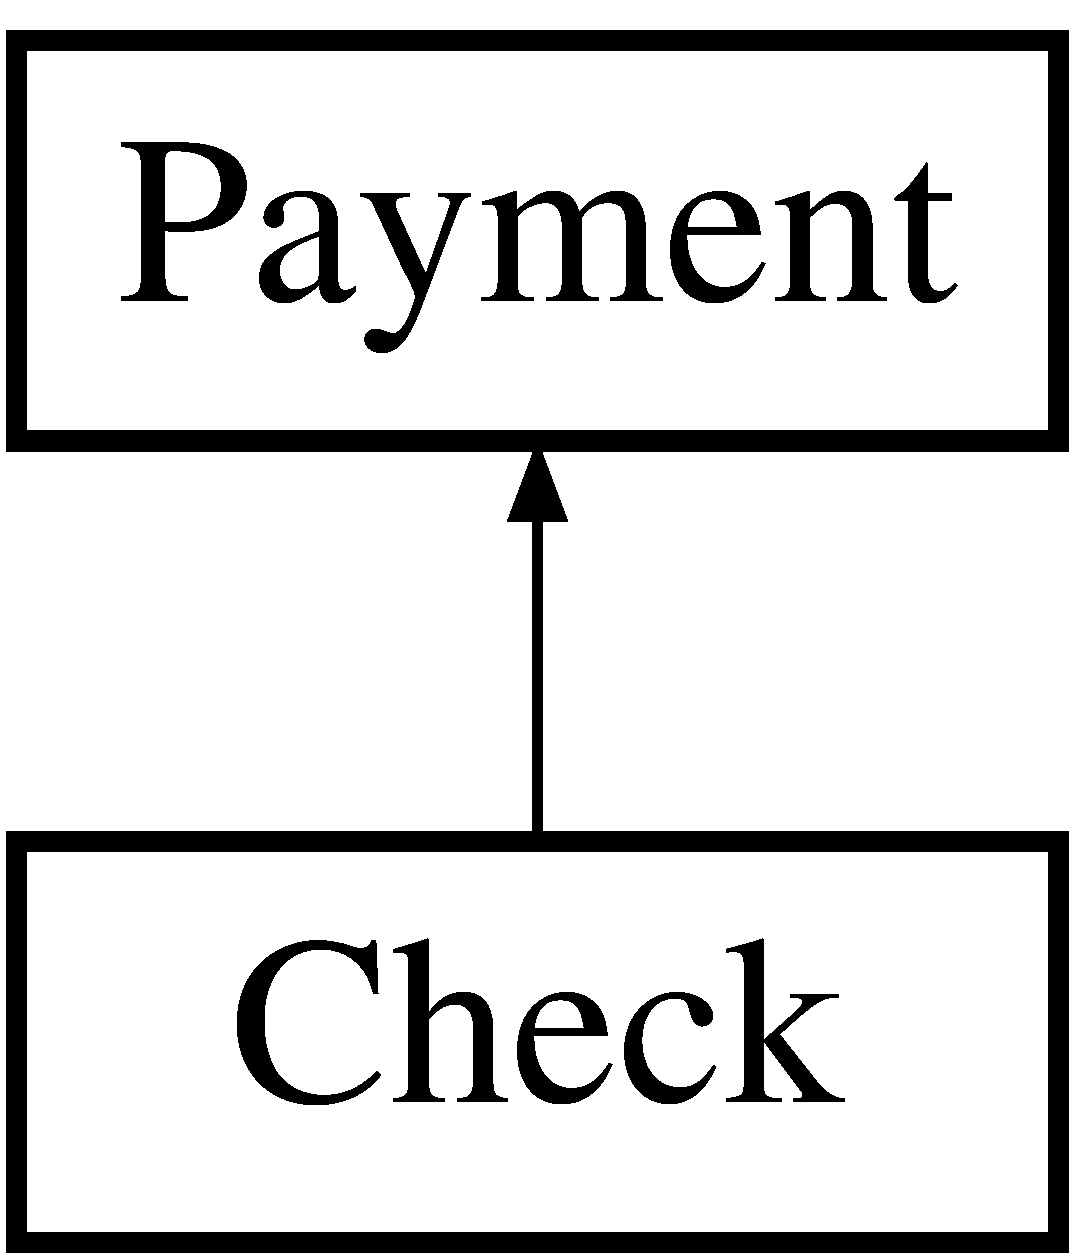
\includegraphics[height=2.000000cm]{classCheck}
\end{center}
\end{figure}
\subsection*{Public Member Functions}
\begin{DoxyCompactItemize}
\item 
\mbox{\Hypertarget{classCheck_af5cce3688521fb9a053211d99c7bef87}\label{classCheck_af5cce3688521fb9a053211d99c7bef87}} 
{\bfseries Check} (double, string, string)
\item 
\mbox{\Hypertarget{classCheck_a494e84c7b7821a3f01d5c80a681490d5}\label{classCheck_a494e84c7b7821a3f01d5c80a681490d5}} 
{\bfseries Check} (double)
\item 
\mbox{\Hypertarget{classCheck_ad69d6ef75ccbb9408f13492fec897c2c}\label{classCheck_ad69d6ef75ccbb9408f13492fec897c2c}} 
string {\bfseries get\+Name} () const
\item 
\mbox{\Hypertarget{classCheck_a84bb7861c25da17be6c5945d48af9415}\label{classCheck_a84bb7861c25da17be6c5945d48af9415}} 
void {\bfseries set\+Name} (string)
\item 
\mbox{\Hypertarget{classCheck_a5e432d25844fafb063cacf4919d23c12}\label{classCheck_a5e432d25844fafb063cacf4919d23c12}} 
string {\bfseries get\+Bank\+ID} () const
\item 
\mbox{\Hypertarget{classCheck_a3b0603c910f0b2395cb472bf903bdee4}\label{classCheck_a3b0603c910f0b2395cb472bf903bdee4}} 
void {\bfseries set\+Bank\+ID} (string)
\item 
\mbox{\Hypertarget{classCheck_adace560cdb9f0faa151b82fe0deb5070}\label{classCheck_adace560cdb9f0faa151b82fe0deb5070}} 
void \hyperlink{classCheck_adace560cdb9f0faa151b82fe0deb5070}{perform\+Payment} ()
\begin{DoxyCompactList}\small\item\em About perform\+Payment. \end{DoxyCompactList}\item 
\mbox{\Hypertarget{classCheck_ab310ce98f6929d4a214c3d120824d2e4}\label{classCheck_ab310ce98f6929d4a214c3d120824d2e4}} 
string \hyperlink{classCheck_ab310ce98f6929d4a214c3d120824d2e4}{payment\+Info} ()
\begin{DoxyCompactList}\small\item\em About payment informations. \end{DoxyCompactList}\end{DoxyCompactItemize}


The documentation for this class was generated from the following files\+:\begin{DoxyCompactItemize}
\item 
Check.\+h\item 
Check.\+cpp\end{DoxyCompactItemize}

\hypertarget{classCreditCard}{}\section{Credit\+Card Class Reference}
\label{classCreditCard}\index{Credit\+Card@{Credit\+Card}}
Inheritance diagram for Credit\+Card\+:\begin{figure}[H]
\begin{center}
\leavevmode
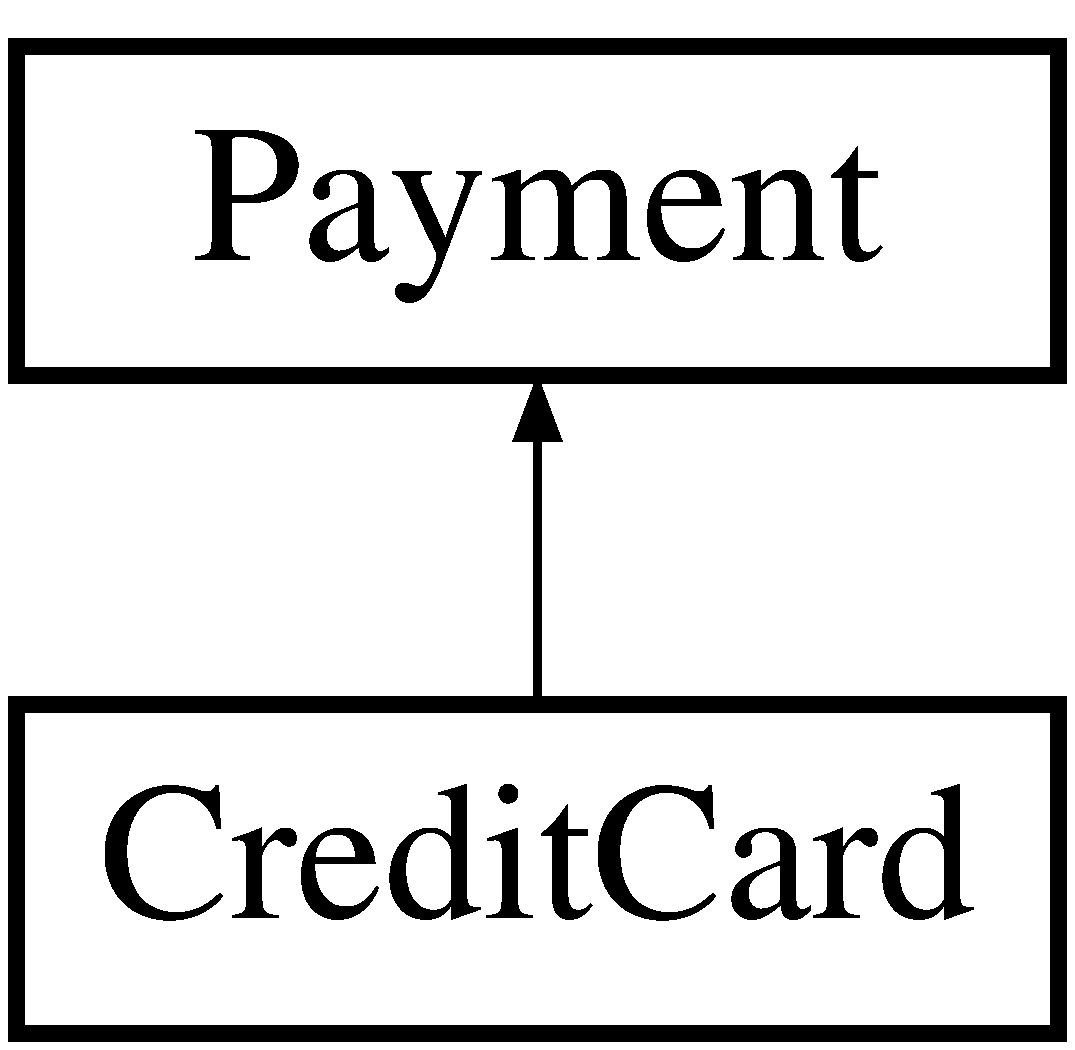
\includegraphics[height=2.000000cm]{classCreditCard}
\end{center}
\end{figure}
\subsection*{Public Member Functions}
\begin{DoxyCompactItemize}
\item 
\mbox{\Hypertarget{classCreditCard_ac44cde50c1d912b02bf147d22da1b117}\label{classCreditCard_ac44cde50c1d912b02bf147d22da1b117}} 
{\bfseries Credit\+Card} (double)
\item 
\mbox{\Hypertarget{classCreditCard_a6d9059ca027aa6ef903158a2efddc35d}\label{classCreditCard_a6d9059ca027aa6ef903158a2efddc35d}} 
{\bfseries Credit\+Card} (double, long, string, string)
\item 
\mbox{\Hypertarget{classCreditCard_a1190bb16e987bc6e0fd37467c30d643b}\label{classCreditCard_a1190bb16e987bc6e0fd37467c30d643b}} 
long {\bfseries get\+Number} () const
\item 
\mbox{\Hypertarget{classCreditCard_aa57cb564e21aef7a8b4f9213f3565992}\label{classCreditCard_aa57cb564e21aef7a8b4f9213f3565992}} 
void {\bfseries set\+Number} (long \+\_\+number)
\item 
\mbox{\Hypertarget{classCreditCard_a7706b969e15ac3e7b4397af600c5024f}\label{classCreditCard_a7706b969e15ac3e7b4397af600c5024f}} 
string {\bfseries get\+Type} () const
\item 
\mbox{\Hypertarget{classCreditCard_a19cc344b1375f7698267999e424eabb3}\label{classCreditCard_a19cc344b1375f7698267999e424eabb3}} 
void {\bfseries set\+Type} (string \+\_\+type)
\item 
\mbox{\Hypertarget{classCreditCard_ad644de7a42046b899b4f2fbb19fd833f}\label{classCreditCard_ad644de7a42046b899b4f2fbb19fd833f}} 
string {\bfseries get\+Exp\+Date} () const
\item 
\mbox{\Hypertarget{classCreditCard_a44c7385c4ed7dbb6f19565c01d84cdd4}\label{classCreditCard_a44c7385c4ed7dbb6f19565c01d84cdd4}} 
void {\bfseries set\+Exp\+Date} (string \+\_\+exp\+Date)
\item 
\mbox{\Hypertarget{classCreditCard_ad41ae39d73adea22555db100311a5101}\label{classCreditCard_ad41ae39d73adea22555db100311a5101}} 
void \hyperlink{classCreditCard_ad41ae39d73adea22555db100311a5101}{perform\+Payment} ()
\begin{DoxyCompactList}\small\item\em About perform\+Payment. \end{DoxyCompactList}\item 
\mbox{\Hypertarget{classCreditCard_af4933bd75406444c8e91d9090b297858}\label{classCreditCard_af4933bd75406444c8e91d9090b297858}} 
string \hyperlink{classCreditCard_af4933bd75406444c8e91d9090b297858}{payment\+Info} ()
\begin{DoxyCompactList}\small\item\em About payment informations. \end{DoxyCompactList}\end{DoxyCompactItemize}


The documentation for this class was generated from the following files\+:\begin{DoxyCompactItemize}
\item 
Credit\+Card.\+h\item 
Credit\+Card.\+cpp\end{DoxyCompactItemize}

\hypertarget{classCustomer}{}\section{Customer Class Reference}
\label{classCustomer}\index{Customer@{Customer}}


\hyperlink{classCustomer}{Customer} class.  




{\ttfamily \#include $<$Customer.\+h$>$}

\subsection*{Public Member Functions}
\begin{DoxyCompactItemize}
\item 
\mbox{\Hypertarget{classCustomer_abcc8fae9701e5ba9d7d6fe44498b34e3}\label{classCustomer_abcc8fae9701e5ba9d7d6fe44498b34e3}} 
\hyperlink{classCustomer_abcc8fae9701e5ba9d7d6fe44498b34e3}{Customer} ()
\begin{DoxyCompactList}\small\item\em Constructor. \end{DoxyCompactList}\item 
\mbox{\Hypertarget{classCustomer_ab93fb14683b0393b9c900109f77c2629}\label{classCustomer_ab93fb14683b0393b9c900109f77c2629}} 
\hyperlink{classCustomer_ab93fb14683b0393b9c900109f77c2629}{$\sim$\+Customer} ()
\begin{DoxyCompactList}\small\item\em Destructor. \end{DoxyCompactList}\item 
\mbox{\Hypertarget{classCustomer_a927d85cfe1f6c23af8dd2a3c73561f49}\label{classCustomer_a927d85cfe1f6c23af8dd2a3c73561f49}} 
void \hyperlink{classCustomer_a927d85cfe1f6c23af8dd2a3c73561f49}{send\+Bill} ()
\begin{DoxyCompactList}\small\item\em Sends bill to adress of the customer. \end{DoxyCompactList}\item 
long \hyperlink{classCustomer_a5c5207f9678017b0fc42ed1f847d288f}{get\+Customer\+ID} () const
\begin{DoxyCompactList}\small\item\em Gets customer\+ID. \end{DoxyCompactList}\item 
void \hyperlink{classCustomer_acc7237a0121638d38846465ee9c2d26a}{set\+Customer\+ID} (long \+\_\+customer\+ID)
\begin{DoxyCompactList}\small\item\em Sets customer\+ID. \end{DoxyCompactList}\item 
string \hyperlink{classCustomer_ac987a032179493e7a75b3dbdc32c1cf9}{get\+Name} () const
\begin{DoxyCompactList}\small\item\em Gets name. \end{DoxyCompactList}\item 
void \hyperlink{classCustomer_a57953fc7e96939d1937fc7603aa31406}{set\+Name} (string \+\_\+name)
\begin{DoxyCompactList}\small\item\em Sets name. \end{DoxyCompactList}\item 
string \hyperlink{classCustomer_a2b0f5ddbc9e4730da690e8cd6391e16e}{get\+Adress} () const
\begin{DoxyCompactList}\small\item\em Gets adress. \end{DoxyCompactList}\item 
void \hyperlink{classCustomer_adfc9ac7abfa4bb4835106dc35739a4a6}{set\+Adress} (string \+\_\+adress)
\begin{DoxyCompactList}\small\item\em Sets adress. \end{DoxyCompactList}\item 
string \hyperlink{classCustomer_ac34eaf091e758c7f8c89f86af2dc29f1}{get\+Phone} () const
\begin{DoxyCompactList}\small\item\em Gets phone. \end{DoxyCompactList}\item 
void \hyperlink{classCustomer_a84e30f04f40a6ef54ec223756b0a59bf}{set\+Phone} (string \+\_\+phone)
\begin{DoxyCompactList}\small\item\em Sets phone. \end{DoxyCompactList}\item 
string \hyperlink{classCustomer_a89fe5dc7065739347c436f673c68b249}{get\+Email} () const
\begin{DoxyCompactList}\small\item\em Gets email. \end{DoxyCompactList}\item 
void \hyperlink{classCustomer_aff04d3f21f7546c394d28f7b42994719}{set\+Email} (string \+\_\+email)
\begin{DoxyCompactList}\small\item\em Sets email. \end{DoxyCompactList}\item 
double \hyperlink{classCustomer_ab4db4b8214793eaf6ddc8597ac8daf1b}{get\+Bonus} () const
\begin{DoxyCompactList}\small\item\em Gets bonus. \end{DoxyCompactList}\item 
void \hyperlink{classCustomer_af983714f01880a3f082c60443fcea84d}{set\+Bonus} (double \+\_\+bonus)
\begin{DoxyCompactList}\small\item\em Sets bonus. \end{DoxyCompactList}\item 
string \hyperlink{classCustomer_aebc1f8d2d749c3f5d132becad88dcbc6}{get\+Username} () const
\begin{DoxyCompactList}\small\item\em Gets username. \end{DoxyCompactList}\item 
void \hyperlink{classCustomer_ab794d5fb843d86eeb79c79dab75302f6}{set\+Username} (string \+\_\+username)
\begin{DoxyCompactList}\small\item\em Sets username. \end{DoxyCompactList}\item 
string \hyperlink{classCustomer_aec5721d16ce287c363cc1aacf5f962fd}{get\+Password} () const
\begin{DoxyCompactList}\small\item\em Gets password. \end{DoxyCompactList}\item 
void \hyperlink{classCustomer_a87953a93ed8a81f9835d26d2ecf3742a}{set\+Password} (string \+\_\+password)
\begin{DoxyCompactList}\small\item\em Sets password. \end{DoxyCompactList}\item 
bool \hyperlink{classCustomer_ae1e9fb03ed6179ecbcd6c0212bc7de17}{check\+Account} (string \+\_\+username, string \+\_\+password)
\begin{DoxyCompactList}\small\item\em Controls input and data, equal or not equal. \end{DoxyCompactList}\item 
void \hyperlink{classCustomer_a6bd365c7ee7c4807de7e0fb94b4a9687}{add\+Bonus} (double \+\_\+bill)
\begin{DoxyCompactList}\small\item\em Adds bill. \end{DoxyCompactList}\item 
void \hyperlink{classCustomer_ab5a0e54395ef83bef1f51a3a98b30ec4}{use\+Bonus} ()
\begin{DoxyCompactList}\small\item\em Uses bonus. \end{DoxyCompactList}\end{DoxyCompactItemize}
\subsection*{Static Public Member Functions}
\begin{DoxyCompactItemize}
\item 
static int \hyperlink{classCustomer_a8bbc27f996653fc209aef876146a2667}{get\+Last\+Id} ()
\begin{DoxyCompactList}\small\item\em Gets last\+Id. \end{DoxyCompactList}\item 
\mbox{\Hypertarget{classCustomer_aaece4550faac5834bc9d7e4158eb1498}\label{classCustomer_aaece4550faac5834bc9d7e4158eb1498}} 
static void \hyperlink{classCustomer_aaece4550faac5834bc9d7e4158eb1498}{set\+Last\+Id} ()
\begin{DoxyCompactList}\small\item\em Increase last\+Id. \end{DoxyCompactList}\end{DoxyCompactItemize}


\subsection{Detailed Description}
\hyperlink{classCustomer}{Customer} class. 

\subsection{Member Function Documentation}
\mbox{\Hypertarget{classCustomer_a6bd365c7ee7c4807de7e0fb94b4a9687}\label{classCustomer_a6bd365c7ee7c4807de7e0fb94b4a9687}} 
\index{Customer@{Customer}!add\+Bonus@{add\+Bonus}}
\index{add\+Bonus@{add\+Bonus}!Customer@{Customer}}
\subsubsection{\texorpdfstring{add\+Bonus()}{addBonus()}}
{\footnotesize\ttfamily void Customer\+::add\+Bonus (\begin{DoxyParamCaption}\item[{double}]{amount }\end{DoxyParamCaption})}



Adds bill. 


\begin{DoxyParams}{Parameters}
{\em amount} & a double argument. \\
\hline
\end{DoxyParams}
\mbox{\Hypertarget{classCustomer_ae1e9fb03ed6179ecbcd6c0212bc7de17}\label{classCustomer_ae1e9fb03ed6179ecbcd6c0212bc7de17}} 
\index{Customer@{Customer}!check\+Account@{check\+Account}}
\index{check\+Account@{check\+Account}!Customer@{Customer}}
\subsubsection{\texorpdfstring{check\+Account()}{checkAccount()}}
{\footnotesize\ttfamily bool Customer\+::check\+Account (\begin{DoxyParamCaption}\item[{string}]{\+\_\+username,  }\item[{string}]{\+\_\+password }\end{DoxyParamCaption})}



Controls input and data, equal or not equal. 

\begin{DoxyReturn}{Returns}
boolean argument. 
\end{DoxyReturn}

\begin{DoxyParams}{Parameters}
{\em username} & a string argument. \\
\hline
{\em password} & a string argument. \\
\hline
\end{DoxyParams}
\mbox{\Hypertarget{classCustomer_a2b0f5ddbc9e4730da690e8cd6391e16e}\label{classCustomer_a2b0f5ddbc9e4730da690e8cd6391e16e}} 
\index{Customer@{Customer}!get\+Adress@{get\+Adress}}
\index{get\+Adress@{get\+Adress}!Customer@{Customer}}
\subsubsection{\texorpdfstring{get\+Adress()}{getAdress()}}
{\footnotesize\ttfamily string Customer\+::get\+Adress (\begin{DoxyParamCaption}{ }\end{DoxyParamCaption}) const}



Gets adress. 

\begin{DoxyReturn}{Returns}
adress a string argument. 
\end{DoxyReturn}
\mbox{\Hypertarget{classCustomer_ab4db4b8214793eaf6ddc8597ac8daf1b}\label{classCustomer_ab4db4b8214793eaf6ddc8597ac8daf1b}} 
\index{Customer@{Customer}!get\+Bonus@{get\+Bonus}}
\index{get\+Bonus@{get\+Bonus}!Customer@{Customer}}
\subsubsection{\texorpdfstring{get\+Bonus()}{getBonus()}}
{\footnotesize\ttfamily double Customer\+::get\+Bonus (\begin{DoxyParamCaption}{ }\end{DoxyParamCaption}) const}



Gets bonus. 

\begin{DoxyReturn}{Returns}
bonus a double argument. 
\end{DoxyReturn}
\mbox{\Hypertarget{classCustomer_a5c5207f9678017b0fc42ed1f847d288f}\label{classCustomer_a5c5207f9678017b0fc42ed1f847d288f}} 
\index{Customer@{Customer}!get\+Customer\+ID@{get\+Customer\+ID}}
\index{get\+Customer\+ID@{get\+Customer\+ID}!Customer@{Customer}}
\subsubsection{\texorpdfstring{get\+Customer\+I\+D()}{getCustomerID()}}
{\footnotesize\ttfamily long Customer\+::get\+Customer\+ID (\begin{DoxyParamCaption}{ }\end{DoxyParamCaption}) const}



Gets customer\+ID. 

\begin{DoxyReturn}{Returns}
customer\+ID a long argument. 
\end{DoxyReturn}
\mbox{\Hypertarget{classCustomer_a89fe5dc7065739347c436f673c68b249}\label{classCustomer_a89fe5dc7065739347c436f673c68b249}} 
\index{Customer@{Customer}!get\+Email@{get\+Email}}
\index{get\+Email@{get\+Email}!Customer@{Customer}}
\subsubsection{\texorpdfstring{get\+Email()}{getEmail()}}
{\footnotesize\ttfamily string Customer\+::get\+Email (\begin{DoxyParamCaption}{ }\end{DoxyParamCaption}) const}



Gets email. 

\begin{DoxyReturn}{Returns}
email a string argument. 
\end{DoxyReturn}
\mbox{\Hypertarget{classCustomer_a8bbc27f996653fc209aef876146a2667}\label{classCustomer_a8bbc27f996653fc209aef876146a2667}} 
\index{Customer@{Customer}!get\+Last\+Id@{get\+Last\+Id}}
\index{get\+Last\+Id@{get\+Last\+Id}!Customer@{Customer}}
\subsubsection{\texorpdfstring{get\+Last\+Id()}{getLastId()}}
{\footnotesize\ttfamily int Customer\+::get\+Last\+Id (\begin{DoxyParamCaption}{ }\end{DoxyParamCaption})\hspace{0.3cm}{\ttfamily [static]}}



Gets last\+Id. 

\begin{DoxyReturn}{Returns}
last\+Id a integer argument. 
\end{DoxyReturn}
\mbox{\Hypertarget{classCustomer_ac987a032179493e7a75b3dbdc32c1cf9}\label{classCustomer_ac987a032179493e7a75b3dbdc32c1cf9}} 
\index{Customer@{Customer}!get\+Name@{get\+Name}}
\index{get\+Name@{get\+Name}!Customer@{Customer}}
\subsubsection{\texorpdfstring{get\+Name()}{getName()}}
{\footnotesize\ttfamily string Customer\+::get\+Name (\begin{DoxyParamCaption}{ }\end{DoxyParamCaption}) const}



Gets name. 

\begin{DoxyReturn}{Returns}
name a string argument. 
\end{DoxyReturn}
\mbox{\Hypertarget{classCustomer_aec5721d16ce287c363cc1aacf5f962fd}\label{classCustomer_aec5721d16ce287c363cc1aacf5f962fd}} 
\index{Customer@{Customer}!get\+Password@{get\+Password}}
\index{get\+Password@{get\+Password}!Customer@{Customer}}
\subsubsection{\texorpdfstring{get\+Password()}{getPassword()}}
{\footnotesize\ttfamily string Customer\+::get\+Password (\begin{DoxyParamCaption}{ }\end{DoxyParamCaption}) const}



Gets password. 

\begin{DoxyReturn}{Returns}
password a string argument. 
\end{DoxyReturn}
\mbox{\Hypertarget{classCustomer_ac34eaf091e758c7f8c89f86af2dc29f1}\label{classCustomer_ac34eaf091e758c7f8c89f86af2dc29f1}} 
\index{Customer@{Customer}!get\+Phone@{get\+Phone}}
\index{get\+Phone@{get\+Phone}!Customer@{Customer}}
\subsubsection{\texorpdfstring{get\+Phone()}{getPhone()}}
{\footnotesize\ttfamily string Customer\+::get\+Phone (\begin{DoxyParamCaption}{ }\end{DoxyParamCaption}) const}



Gets phone. 

\begin{DoxyReturn}{Returns}
phone a string argument. 
\end{DoxyReturn}
\mbox{\Hypertarget{classCustomer_aebc1f8d2d749c3f5d132becad88dcbc6}\label{classCustomer_aebc1f8d2d749c3f5d132becad88dcbc6}} 
\index{Customer@{Customer}!get\+Username@{get\+Username}}
\index{get\+Username@{get\+Username}!Customer@{Customer}}
\subsubsection{\texorpdfstring{get\+Username()}{getUsername()}}
{\footnotesize\ttfamily string Customer\+::get\+Username (\begin{DoxyParamCaption}{ }\end{DoxyParamCaption}) const}



Gets username. 

\begin{DoxyReturn}{Returns}
username a string argument. 
\end{DoxyReturn}
\mbox{\Hypertarget{classCustomer_adfc9ac7abfa4bb4835106dc35739a4a6}\label{classCustomer_adfc9ac7abfa4bb4835106dc35739a4a6}} 
\index{Customer@{Customer}!set\+Adress@{set\+Adress}}
\index{set\+Adress@{set\+Adress}!Customer@{Customer}}
\subsubsection{\texorpdfstring{set\+Adress()}{setAdress()}}
{\footnotesize\ttfamily void Customer\+::set\+Adress (\begin{DoxyParamCaption}\item[{string}]{\+\_\+adress }\end{DoxyParamCaption})}



Sets adress. 


\begin{DoxyParams}{Parameters}
{\em adress} & a string argument. \\
\hline
\end{DoxyParams}
\mbox{\Hypertarget{classCustomer_af983714f01880a3f082c60443fcea84d}\label{classCustomer_af983714f01880a3f082c60443fcea84d}} 
\index{Customer@{Customer}!set\+Bonus@{set\+Bonus}}
\index{set\+Bonus@{set\+Bonus}!Customer@{Customer}}
\subsubsection{\texorpdfstring{set\+Bonus()}{setBonus()}}
{\footnotesize\ttfamily void Customer\+::set\+Bonus (\begin{DoxyParamCaption}\item[{double}]{\+\_\+bonus }\end{DoxyParamCaption})}



Sets bonus. 


\begin{DoxyParams}{Parameters}
{\em bonus} & a double argument. \\
\hline
\end{DoxyParams}
\mbox{\Hypertarget{classCustomer_acc7237a0121638d38846465ee9c2d26a}\label{classCustomer_acc7237a0121638d38846465ee9c2d26a}} 
\index{Customer@{Customer}!set\+Customer\+ID@{set\+Customer\+ID}}
\index{set\+Customer\+ID@{set\+Customer\+ID}!Customer@{Customer}}
\subsubsection{\texorpdfstring{set\+Customer\+I\+D()}{setCustomerID()}}
{\footnotesize\ttfamily void Customer\+::set\+Customer\+ID (\begin{DoxyParamCaption}\item[{long}]{\+\_\+customer\+ID }\end{DoxyParamCaption})}



Sets customer\+ID. 


\begin{DoxyParams}{Parameters}
{\em customer\+ID} & a long argument. \\
\hline
\end{DoxyParams}
\mbox{\Hypertarget{classCustomer_aff04d3f21f7546c394d28f7b42994719}\label{classCustomer_aff04d3f21f7546c394d28f7b42994719}} 
\index{Customer@{Customer}!set\+Email@{set\+Email}}
\index{set\+Email@{set\+Email}!Customer@{Customer}}
\subsubsection{\texorpdfstring{set\+Email()}{setEmail()}}
{\footnotesize\ttfamily void Customer\+::set\+Email (\begin{DoxyParamCaption}\item[{string}]{\+\_\+email }\end{DoxyParamCaption})}



Sets email. 


\begin{DoxyParams}{Parameters}
{\em email} & a string argument. \\
\hline
\end{DoxyParams}
\mbox{\Hypertarget{classCustomer_a57953fc7e96939d1937fc7603aa31406}\label{classCustomer_a57953fc7e96939d1937fc7603aa31406}} 
\index{Customer@{Customer}!set\+Name@{set\+Name}}
\index{set\+Name@{set\+Name}!Customer@{Customer}}
\subsubsection{\texorpdfstring{set\+Name()}{setName()}}
{\footnotesize\ttfamily void Customer\+::set\+Name (\begin{DoxyParamCaption}\item[{string}]{\+\_\+name }\end{DoxyParamCaption})}



Sets name. 


\begin{DoxyParams}{Parameters}
{\em name} & a string argument. \\
\hline
\end{DoxyParams}
\mbox{\Hypertarget{classCustomer_a87953a93ed8a81f9835d26d2ecf3742a}\label{classCustomer_a87953a93ed8a81f9835d26d2ecf3742a}} 
\index{Customer@{Customer}!set\+Password@{set\+Password}}
\index{set\+Password@{set\+Password}!Customer@{Customer}}
\subsubsection{\texorpdfstring{set\+Password()}{setPassword()}}
{\footnotesize\ttfamily void Customer\+::set\+Password (\begin{DoxyParamCaption}\item[{string}]{\+\_\+password }\end{DoxyParamCaption})}



Sets password. 


\begin{DoxyParams}{Parameters}
{\em password} & a string argument. \\
\hline
\end{DoxyParams}
\mbox{\Hypertarget{classCustomer_a84e30f04f40a6ef54ec223756b0a59bf}\label{classCustomer_a84e30f04f40a6ef54ec223756b0a59bf}} 
\index{Customer@{Customer}!set\+Phone@{set\+Phone}}
\index{set\+Phone@{set\+Phone}!Customer@{Customer}}
\subsubsection{\texorpdfstring{set\+Phone()}{setPhone()}}
{\footnotesize\ttfamily void Customer\+::set\+Phone (\begin{DoxyParamCaption}\item[{string}]{\+\_\+phone }\end{DoxyParamCaption})}



Sets phone. 


\begin{DoxyParams}{Parameters}
{\em phone} & a string argument. \\
\hline
\end{DoxyParams}
\mbox{\Hypertarget{classCustomer_ab794d5fb843d86eeb79c79dab75302f6}\label{classCustomer_ab794d5fb843d86eeb79c79dab75302f6}} 
\index{Customer@{Customer}!set\+Username@{set\+Username}}
\index{set\+Username@{set\+Username}!Customer@{Customer}}
\subsubsection{\texorpdfstring{set\+Username()}{setUsername()}}
{\footnotesize\ttfamily void Customer\+::set\+Username (\begin{DoxyParamCaption}\item[{string}]{\+\_\+username }\end{DoxyParamCaption})}



Sets username. 


\begin{DoxyParams}{Parameters}
{\em username} & a string argument. \\
\hline
\end{DoxyParams}
\mbox{\Hypertarget{classCustomer_ab5a0e54395ef83bef1f51a3a98b30ec4}\label{classCustomer_ab5a0e54395ef83bef1f51a3a98b30ec4}} 
\index{Customer@{Customer}!use\+Bonus@{use\+Bonus}}
\index{use\+Bonus@{use\+Bonus}!Customer@{Customer}}
\subsubsection{\texorpdfstring{use\+Bonus()}{useBonus()}}
{\footnotesize\ttfamily void Customer\+::use\+Bonus (\begin{DoxyParamCaption}{ }\end{DoxyParamCaption})}



Uses bonus. 


\begin{DoxyParams}{Parameters}
{\em amount} & a double argument. \\
\hline
\end{DoxyParams}


The documentation for this class was generated from the following files\+:\begin{DoxyCompactItemize}
\item 
Customer.\+h\item 
Customer.\+cpp\end{DoxyCompactItemize}

\hypertarget{classCustomerMenu}{}\section{Customer\+Menu Class Reference}
\label{classCustomerMenu}\index{Customer\+Menu@{Customer\+Menu}}


\hyperlink{classCustomerMenu}{Customer\+Menu} class.  




{\ttfamily \#include $<$Customer\+Menu.\+h$>$}

Inheritance diagram for Customer\+Menu\+:\begin{figure}[H]
\begin{center}
\leavevmode
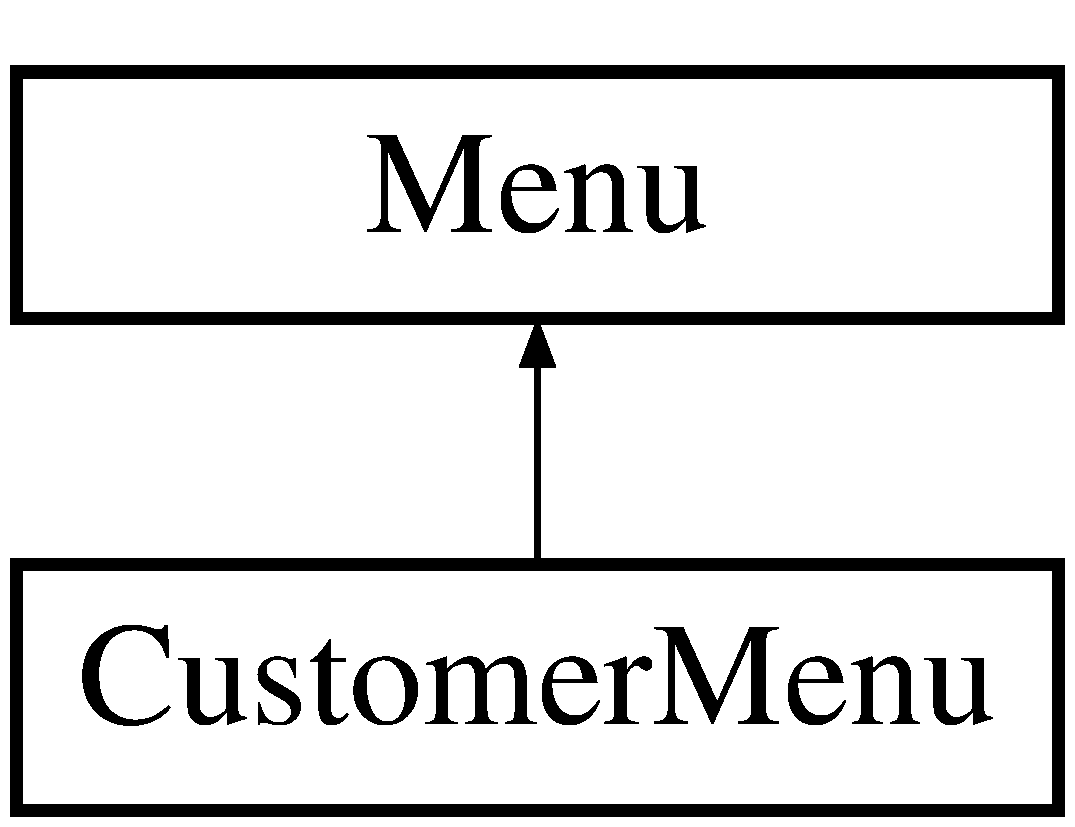
\includegraphics[height=2.000000cm]{classCustomerMenu}
\end{center}
\end{figure}
\subsection*{Public Member Functions}
\begin{DoxyCompactItemize}
\item 
\mbox{\Hypertarget{classCustomerMenu_a05bf66ccf5ce81d26cc4e39fbc2dbb64}\label{classCustomerMenu_a05bf66ccf5ce81d26cc4e39fbc2dbb64}} 
\hyperlink{classCustomerMenu_a05bf66ccf5ce81d26cc4e39fbc2dbb64}{Customer\+Menu} (string title, string $\ast$subs, int size, vector$<$ \hyperlink{classCustomer}{Customer} $>$ c\+List)
\begin{DoxyCompactList}\small\item\em Constructor. \end{DoxyCompactList}\item 
void \hyperlink{classCustomerMenu_abd785329cc569b15848388dd9e193613}{set\+Customer\+List} (const vector$<$ \hyperlink{classCustomer}{Customer} $>$ \&customer\+List)
\begin{DoxyCompactList}\small\item\em Sets customer\+List. \end{DoxyCompactList}\item 
const vector$<$ \hyperlink{classCustomer}{Customer} $>$ \& \hyperlink{classCustomerMenu_a633a6392060ef6e6bdb94ea6d554429c}{get\+Customer\+List} () const
\begin{DoxyCompactList}\small\item\em Gets customer\+List. \end{DoxyCompactList}\item 
\hyperlink{classCustomerMenu_aa28a689d645c7df53e2d714195fcf08e}{$\sim$\+Customer\+Menu} ()
\begin{DoxyCompactList}\small\item\em Destructor. \end{DoxyCompactList}\item 
void \hyperlink{classCustomerMenu_a9c43057a2fdd5fa1323e4cc1ec54f4be}{menu\+Switch} (int)
\begin{DoxyCompactList}\small\item\em Switchs menu by input. \end{DoxyCompactList}\end{DoxyCompactItemize}
\subsection*{Additional Inherited Members}


\subsection{Detailed Description}
\hyperlink{classCustomerMenu}{Customer\+Menu} class. 

\hyperlink{classCustomerMenu}{Customer\+Menu} class inherits from menu class. 

\subsection{Constructor \& Destructor Documentation}
\mbox{\Hypertarget{classCustomerMenu_aa28a689d645c7df53e2d714195fcf08e}\label{classCustomerMenu_aa28a689d645c7df53e2d714195fcf08e}} 
\index{Customer\+Menu@{Customer\+Menu}!````~Customer\+Menu@{$\sim$\+Customer\+Menu}}
\index{````~Customer\+Menu@{$\sim$\+Customer\+Menu}!Customer\+Menu@{Customer\+Menu}}
\subsubsection{\texorpdfstring{$\sim$\+Customer\+Menu()}{~CustomerMenu()}}
{\footnotesize\ttfamily Customer\+Menu\+::$\sim$\+Customer\+Menu (\begin{DoxyParamCaption}{ }\end{DoxyParamCaption})}



Destructor. 

\hyperlink{classCustomerMenu}{Customer\+Menu} class. 

\subsection{Member Function Documentation}
\mbox{\Hypertarget{classCustomerMenu_a633a6392060ef6e6bdb94ea6d554429c}\label{classCustomerMenu_a633a6392060ef6e6bdb94ea6d554429c}} 
\index{Customer\+Menu@{Customer\+Menu}!get\+Customer\+List@{get\+Customer\+List}}
\index{get\+Customer\+List@{get\+Customer\+List}!Customer\+Menu@{Customer\+Menu}}
\subsubsection{\texorpdfstring{get\+Customer\+List()}{getCustomerList()}}
{\footnotesize\ttfamily const vector$<$ \hyperlink{classCustomer}{Customer} $>$ \& Customer\+Menu\+::get\+Customer\+List (\begin{DoxyParamCaption}{ }\end{DoxyParamCaption}) const}



Gets customer\+List. 

\begin{DoxyReturn}{Returns}
customer\+List a customer argument. 
\end{DoxyReturn}
\mbox{\Hypertarget{classCustomerMenu_a9c43057a2fdd5fa1323e4cc1ec54f4be}\label{classCustomerMenu_a9c43057a2fdd5fa1323e4cc1ec54f4be}} 
\index{Customer\+Menu@{Customer\+Menu}!menu\+Switch@{menu\+Switch}}
\index{menu\+Switch@{menu\+Switch}!Customer\+Menu@{Customer\+Menu}}
\subsubsection{\texorpdfstring{menu\+Switch()}{menuSwitch()}}
{\footnotesize\ttfamily void Customer\+Menu\+::menu\+Switch (\begin{DoxyParamCaption}\item[{int}]{menu\+Input }\end{DoxyParamCaption})\hspace{0.3cm}{\ttfamily [virtual]}}



Switchs menu by input. 


\begin{DoxyParams}{Parameters}
{\em menu\+Input} & an integer argument. \\
\hline
\end{DoxyParams}


Implements \hyperlink{classMenu_ae9d7af36b1a380e5e4b03ddbef9ceeca}{Menu}.

\mbox{\Hypertarget{classCustomerMenu_abd785329cc569b15848388dd9e193613}\label{classCustomerMenu_abd785329cc569b15848388dd9e193613}} 
\index{Customer\+Menu@{Customer\+Menu}!set\+Customer\+List@{set\+Customer\+List}}
\index{set\+Customer\+List@{set\+Customer\+List}!Customer\+Menu@{Customer\+Menu}}
\subsubsection{\texorpdfstring{set\+Customer\+List()}{setCustomerList()}}
{\footnotesize\ttfamily void Customer\+Menu\+::set\+Customer\+List (\begin{DoxyParamCaption}\item[{const vector$<$ \hyperlink{classCustomer}{Customer} $>$ \&}]{customer\+List }\end{DoxyParamCaption})}



Sets customer\+List. 


\begin{DoxyParams}{Parameters}
{\em customer\+List} & a customer argument. \\
\hline
\end{DoxyParams}


The documentation for this class was generated from the following files\+:\begin{DoxyCompactItemize}
\item 
Customer\+Menu.\+h\item 
Customer\+Menu.\+cpp\end{DoxyCompactItemize}

\hypertarget{classMagazine}{}\section{Magazine Class Reference}
\label{classMagazine}\index{Magazine@{Magazine}}


\hyperlink{classMagazine}{Magazine} class inherits from product class.  




{\ttfamily \#include $<$Magazine.\+h$>$}

Inheritance diagram for Magazine\+:\begin{figure}[H]
\begin{center}
\leavevmode
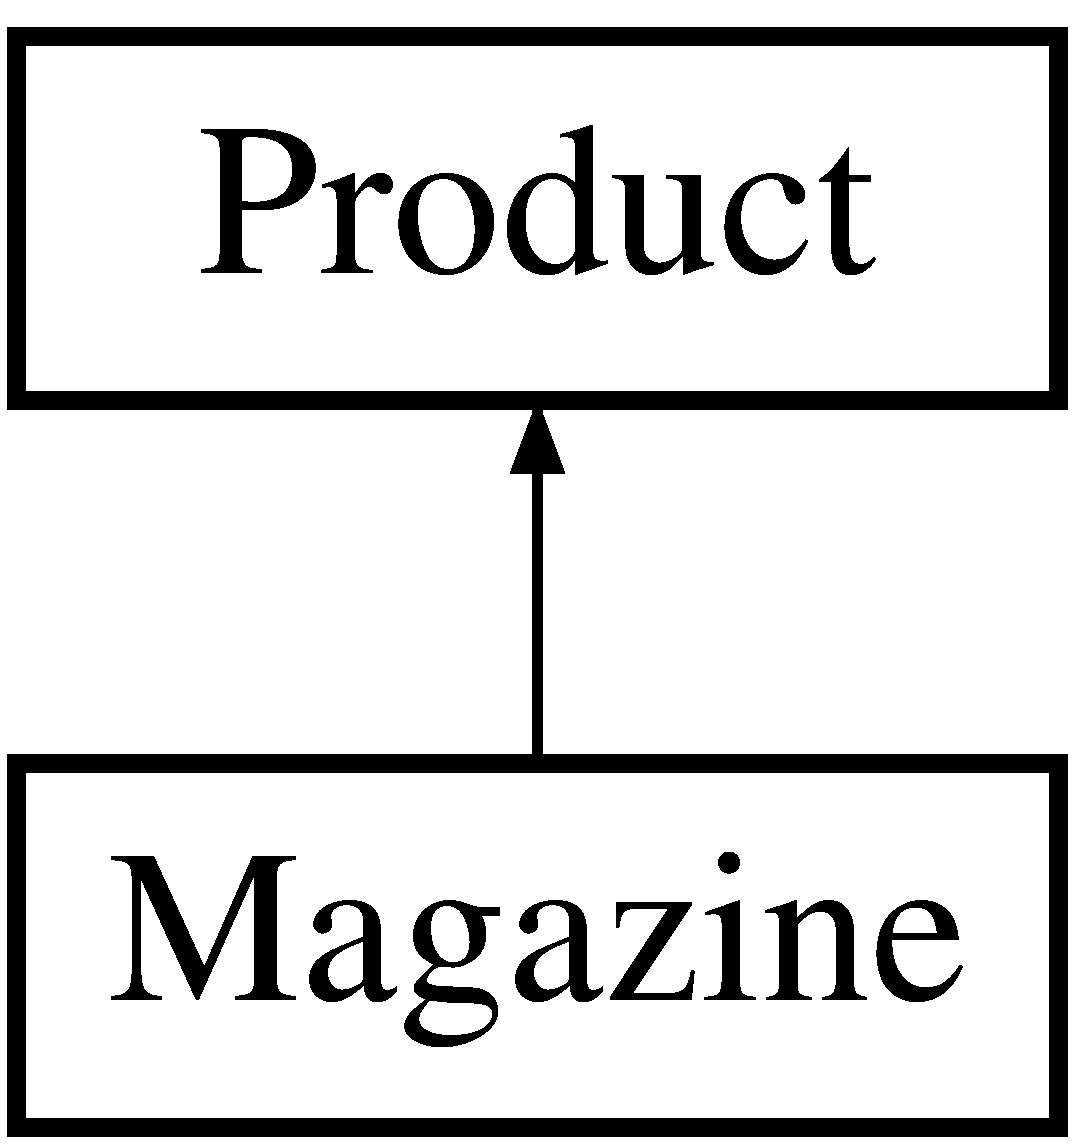
\includegraphics[height=2.000000cm]{classMagazine}
\end{center}
\end{figure}
\subsection*{Public Member Functions}
\begin{DoxyCompactItemize}
\item 
\hyperlink{classMagazine_af32c7b2b56f8553579669f9f3200e2e7}{Magazine} (int, string, double, int, string)
\begin{DoxyCompactList}\small\item\em Constructor with five arguments. \end{DoxyCompactList}\item 
\hyperlink{classMagazine_ad79b115f747f89d5f1cebe268a94e0cb}{Magazine} (int, string, double)
\begin{DoxyCompactList}\small\item\em Constructor with three arguments. \end{DoxyCompactList}\item 
\mbox{\Hypertarget{classMagazine_a0ba688d442bd6666825132522049da05}\label{classMagazine_a0ba688d442bd6666825132522049da05}} 
virtual \hyperlink{classMagazine_a0ba688d442bd6666825132522049da05}{$\sim$\+Magazine} ()
\begin{DoxyCompactList}\small\item\em Destructor. \end{DoxyCompactList}\item 
\mbox{\Hypertarget{classMagazine_a64f61943072de7e5c608a52cf5ee86ac}\label{classMagazine_a64f61943072de7e5c608a52cf5ee86ac}} 
void \hyperlink{classMagazine_a64f61943072de7e5c608a52cf5ee86ac}{print\+Properties} ()
\begin{DoxyCompactList}\small\item\em Prints the properties. \end{DoxyCompactList}\item 
int \hyperlink{classMagazine_a15d88a272355e02568dab18f3df0934a}{get\+Issue} () const
\begin{DoxyCompactList}\small\item\em Gets issue.\+return issue. \end{DoxyCompactList}\item 
void \hyperlink{classMagazine_a19df08bb3f6848601a04f03486d57099}{set\+Issue} (int)
\begin{DoxyCompactList}\small\item\em Sets issue\+Parameter. \end{DoxyCompactList}\item 
string \hyperlink{classMagazine_a46f8e02963fc1c130cc1b3e1f0e67e30}{get\+Type} () const
\begin{DoxyCompactList}\small\item\em Gets type. \end{DoxyCompactList}\item 
void \hyperlink{classMagazine_a29b2f7bd3ec5a76e9a5b0d06d64dec68}{set\+Type} (string)
\begin{DoxyCompactList}\small\item\em Sets type. \end{DoxyCompactList}\end{DoxyCompactItemize}


\subsection{Detailed Description}
\hyperlink{classMagazine}{Magazine} class inherits from product class. 

\subsection{Constructor \& Destructor Documentation}
\mbox{\Hypertarget{classMagazine_af32c7b2b56f8553579669f9f3200e2e7}\label{classMagazine_af32c7b2b56f8553579669f9f3200e2e7}} 
\index{Magazine@{Magazine}!Magazine@{Magazine}}
\index{Magazine@{Magazine}!Magazine@{Magazine}}
\subsubsection{\texorpdfstring{Magazine()}{Magazine()}\hspace{0.1cm}{\footnotesize\ttfamily [1/2]}}
{\footnotesize\ttfamily Magazine\+::\+Magazine (\begin{DoxyParamCaption}\item[{int}]{id,  }\item[{string}]{name,  }\item[{double}]{price,  }\item[{int}]{Issue,  }\item[{string}]{type }\end{DoxyParamCaption})}



Constructor with five arguments. 


\begin{DoxyParams}{Parameters}
{\em id} & an integer argument. \\
\hline
{\em name} & a string argument. \\
\hline
{\em price} & a double argument. \\
\hline
{\em issue} & an integer argument. \\
\hline
{\em type} & a string argument. \\
\hline
\end{DoxyParams}
\mbox{\Hypertarget{classMagazine_ad79b115f747f89d5f1cebe268a94e0cb}\label{classMagazine_ad79b115f747f89d5f1cebe268a94e0cb}} 
\index{Magazine@{Magazine}!Magazine@{Magazine}}
\index{Magazine@{Magazine}!Magazine@{Magazine}}
\subsubsection{\texorpdfstring{Magazine()}{Magazine()}\hspace{0.1cm}{\footnotesize\ttfamily [2/2]}}
{\footnotesize\ttfamily Magazine\+::\+Magazine (\begin{DoxyParamCaption}\item[{int}]{id,  }\item[{string}]{name,  }\item[{double}]{price }\end{DoxyParamCaption})}



Constructor with three arguments. 


\begin{DoxyParams}{Parameters}
{\em id} & an integer argument. \\
\hline
{\em name} & a string argument. \\
\hline
{\em price} & a double argument. \\
\hline
\end{DoxyParams}


\subsection{Member Function Documentation}
\mbox{\Hypertarget{classMagazine_a15d88a272355e02568dab18f3df0934a}\label{classMagazine_a15d88a272355e02568dab18f3df0934a}} 
\index{Magazine@{Magazine}!get\+Issue@{get\+Issue}}
\index{get\+Issue@{get\+Issue}!Magazine@{Magazine}}
\subsubsection{\texorpdfstring{get\+Issue()}{getIssue()}}
{\footnotesize\ttfamily int Magazine\+::get\+Issue (\begin{DoxyParamCaption}{ }\end{DoxyParamCaption}) const}



Gets issue.\+return issue. 

\hyperlink{classCustomerMenu}{Customer\+Menu} class.

\begin{DoxyReturn}{Returns}
issue an integer argument. 
\end{DoxyReturn}
\mbox{\Hypertarget{classMagazine_a46f8e02963fc1c130cc1b3e1f0e67e30}\label{classMagazine_a46f8e02963fc1c130cc1b3e1f0e67e30}} 
\index{Magazine@{Magazine}!get\+Type@{get\+Type}}
\index{get\+Type@{get\+Type}!Magazine@{Magazine}}
\subsubsection{\texorpdfstring{get\+Type()}{getType()}}
{\footnotesize\ttfamily string Magazine\+::get\+Type (\begin{DoxyParamCaption}{ }\end{DoxyParamCaption}) const}



Gets type. 

\begin{DoxyReturn}{Returns}
type a string argument. 
\end{DoxyReturn}
\mbox{\Hypertarget{classMagazine_a19df08bb3f6848601a04f03486d57099}\label{classMagazine_a19df08bb3f6848601a04f03486d57099}} 
\index{Magazine@{Magazine}!set\+Issue@{set\+Issue}}
\index{set\+Issue@{set\+Issue}!Magazine@{Magazine}}
\subsubsection{\texorpdfstring{set\+Issue()}{setIssue()}}
{\footnotesize\ttfamily void Magazine\+::set\+Issue (\begin{DoxyParamCaption}\item[{int}]{ }\end{DoxyParamCaption})}



Sets issue\+Parameter. 


\begin{DoxyParams}{Parameters}
{\em issue} & an integer argument. \\
\hline
\end{DoxyParams}
\mbox{\Hypertarget{classMagazine_a29b2f7bd3ec5a76e9a5b0d06d64dec68}\label{classMagazine_a29b2f7bd3ec5a76e9a5b0d06d64dec68}} 
\index{Magazine@{Magazine}!set\+Type@{set\+Type}}
\index{set\+Type@{set\+Type}!Magazine@{Magazine}}
\subsubsection{\texorpdfstring{set\+Type()}{setType()}}
{\footnotesize\ttfamily void Magazine\+::set\+Type (\begin{DoxyParamCaption}\item[{string}]{ }\end{DoxyParamCaption})}



Sets type. 


\begin{DoxyParams}{Parameters}
{\em type} & a string argument. \\
\hline
\end{DoxyParams}


The documentation for this class was generated from the following files\+:\begin{DoxyCompactItemize}
\item 
Magazine.\+h\item 
Magazine.\+cpp\end{DoxyCompactItemize}

\hypertarget{classMainMenu}{}\section{Main\+Menu Class Reference}
\label{classMainMenu}\index{Main\+Menu@{Main\+Menu}}


\hyperlink{classMainMenu}{Main\+Menu} class.  




{\ttfamily \#include $<$Main\+Menu.\+h$>$}

Inheritance diagram for Main\+Menu\+:\begin{figure}[H]
\begin{center}
\leavevmode
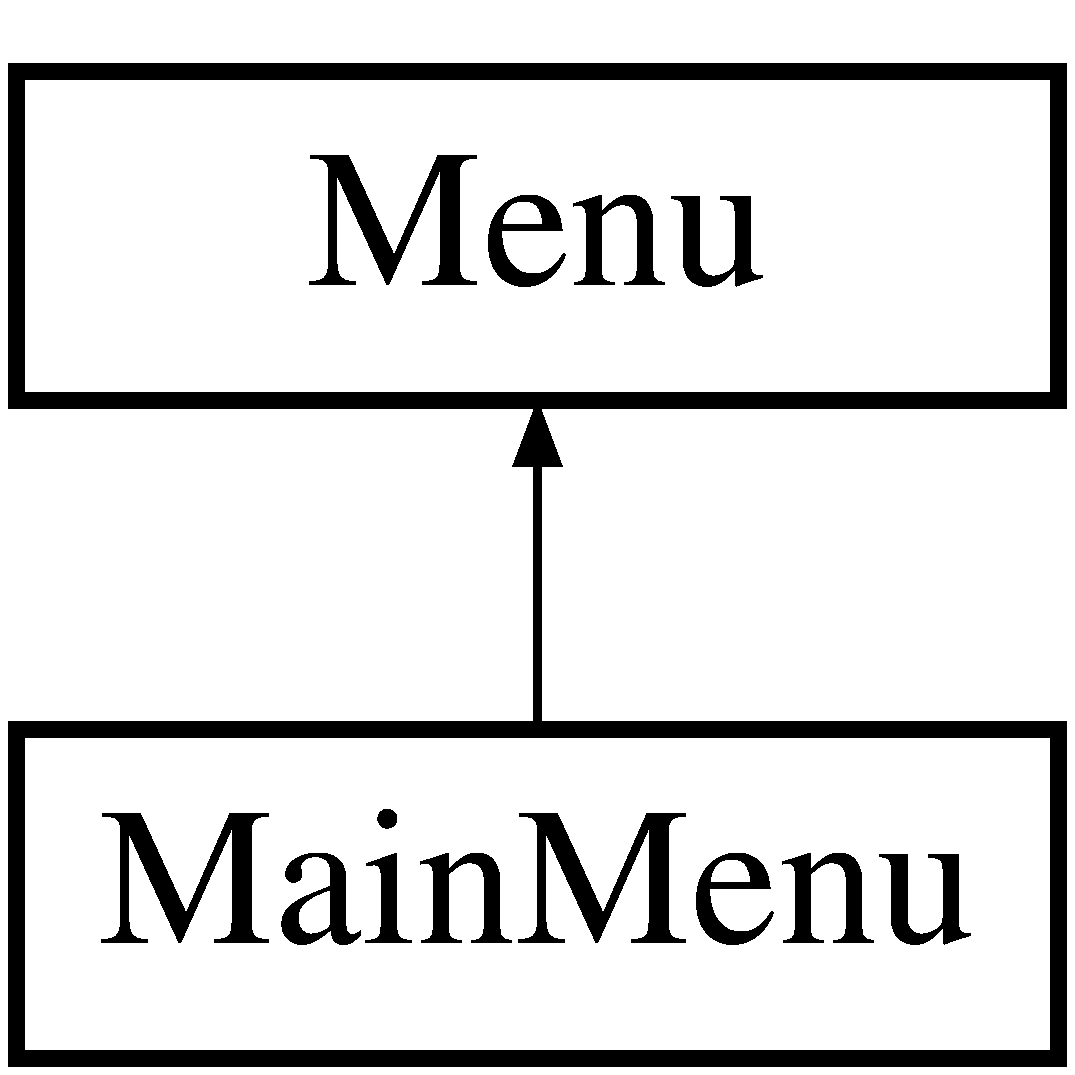
\includegraphics[height=2.000000cm]{classMainMenu}
\end{center}
\end{figure}
\subsection*{Public Member Functions}
\begin{DoxyCompactItemize}
\item 
const vector$<$ \hyperlink{classProduct}{Product} $\ast$ $>$ \& \hyperlink{classMainMenu_ae122d42a6ffd8735c4abcd789473a4e9}{get\+Product\+List} () const
\begin{DoxyCompactList}\small\item\em Gets product\+List. \end{DoxyCompactList}\item 
const vector$<$ \hyperlink{classCustomer}{Customer} $>$ \& \hyperlink{classMainMenu_ac1e7ab45aeaf1245b7dd534e2a535ed8}{get\+Customer\+List} () const
\begin{DoxyCompactList}\small\item\em Gets customer\+List. \end{DoxyCompactList}\item 
void \hyperlink{classMainMenu_aae749e64ea9bf630ae4340a446bcf8a7}{set\+Product\+List} (const vector$<$ \hyperlink{classProduct}{Product} $\ast$$>$ \&product\+List)
\begin{DoxyCompactList}\small\item\em Sets product\+List. \end{DoxyCompactList}\item 
void \hyperlink{classMainMenu_aa78eaffbe8203475575aac6f330497c9}{set\+Customer\+List} (const vector$<$ \hyperlink{classCustomer}{Customer} $>$ \&customer\+List)
\begin{DoxyCompactList}\small\item\em Sets customer\+List. \end{DoxyCompactList}\item 
\hyperlink{classProductMenu}{Product\+Menu} $\ast$ \hyperlink{classMainMenu_a96cf34491424fb414023b2ae6f64540b}{get\+Product\+Menu} () const
\begin{DoxyCompactList}\small\item\em Gets product\+Menu. \end{DoxyCompactList}\item 
void \hyperlink{classMainMenu_aaca12cbc08bfe9533544375cd8da5a8e}{set\+Product\+Menu} (\hyperlink{classProductMenu}{Product\+Menu} $\ast$product\+Menu)
\begin{DoxyCompactList}\small\item\em Sets product\+Menu. \end{DoxyCompactList}\item 
\hyperlink{classShoppingMenu}{Shopping\+Menu} $\ast$ \hyperlink{classMainMenu_a59f7c25cfd99dc969de1b29acda75a9c}{get\+Shopping\+Menu} () const
\begin{DoxyCompactList}\small\item\em Gets shopping\+Menu. \end{DoxyCompactList}\item 
void \hyperlink{classMainMenu_ae8cab8d0e2430d34bad64ba238b4cc4d}{set\+Shopping\+Menu} (\hyperlink{classShoppingMenu}{Shopping\+Menu} $\ast$shopping\+Menu)
\begin{DoxyCompactList}\small\item\em Sets shopping\+Menu. \end{DoxyCompactList}\item 
\hyperlink{classCustomerMenu}{Customer\+Menu} $\ast$ \hyperlink{classMainMenu_a605159269deb516a64b77d9144750bbf}{get\+Customer\+Menu} () const
\begin{DoxyCompactList}\small\item\em Gets customer\+Menu. \end{DoxyCompactList}\item 
void \hyperlink{classMainMenu_a5c80f2e447ac6fca73b1527f9abd74b6}{set\+Customer\+Menu} (\hyperlink{classCustomerMenu}{Customer\+Menu} $\ast$customer\+Menu)
\begin{DoxyCompactList}\small\item\em Sets customer\+Menu. \end{DoxyCompactList}\item 
void \hyperlink{classMainMenu_aabbf0c8aba7bc80316e150ea609e897f}{menu\+Switch} (int)
\begin{DoxyCompactList}\small\item\em Switchs to menu. \end{DoxyCompactList}\end{DoxyCompactItemize}
\subsection*{Public Attributes}
\begin{DoxyCompactItemize}
\item 
\hyperlink{classMainMenu}{Main\+Menu}(string title, string $\ast$subs, int size \hyperlink{classMainMenu_a70561c3a6ca04aaa2d7a28d4b157a462}{$\sim$\+Main\+Menu} )()
\begin{DoxyCompactList}\small\item\em Constructor with six arguments. \end{DoxyCompactList}\end{DoxyCompactItemize}
\subsection*{Additional Inherited Members}


\subsection{Detailed Description}
\hyperlink{classMainMenu}{Main\+Menu} class. 

\hyperlink{classMainMenu}{Main\+Menu} class inherits from menu class. 

\subsection{Member Function Documentation}
\mbox{\Hypertarget{classMainMenu_ac1e7ab45aeaf1245b7dd534e2a535ed8}\label{classMainMenu_ac1e7ab45aeaf1245b7dd534e2a535ed8}} 
\index{Main\+Menu@{Main\+Menu}!get\+Customer\+List@{get\+Customer\+List}}
\index{get\+Customer\+List@{get\+Customer\+List}!Main\+Menu@{Main\+Menu}}
\subsubsection{\texorpdfstring{get\+Customer\+List()}{getCustomerList()}}
{\footnotesize\ttfamily const vector$<$ \hyperlink{classCustomer}{Customer} $>$ \& Main\+Menu\+::get\+Customer\+List (\begin{DoxyParamCaption}{ }\end{DoxyParamCaption}) const}



Gets customer\+List. 

\begin{DoxyReturn}{Returns}
customer\+List a customer argument. 
\end{DoxyReturn}
\mbox{\Hypertarget{classMainMenu_a605159269deb516a64b77d9144750bbf}\label{classMainMenu_a605159269deb516a64b77d9144750bbf}} 
\index{Main\+Menu@{Main\+Menu}!get\+Customer\+Menu@{get\+Customer\+Menu}}
\index{get\+Customer\+Menu@{get\+Customer\+Menu}!Main\+Menu@{Main\+Menu}}
\subsubsection{\texorpdfstring{get\+Customer\+Menu()}{getCustomerMenu()}}
{\footnotesize\ttfamily \hyperlink{classCustomerMenu}{Customer\+Menu} $\ast$ Main\+Menu\+::get\+Customer\+Menu (\begin{DoxyParamCaption}{ }\end{DoxyParamCaption}) const}



Gets customer\+Menu. 

\begin{DoxyReturn}{Returns}
customer\+Menu a \hyperlink{classCustomerMenu}{Customer\+Menu} argument. 
\end{DoxyReturn}
\mbox{\Hypertarget{classMainMenu_ae122d42a6ffd8735c4abcd789473a4e9}\label{classMainMenu_ae122d42a6ffd8735c4abcd789473a4e9}} 
\index{Main\+Menu@{Main\+Menu}!get\+Product\+List@{get\+Product\+List}}
\index{get\+Product\+List@{get\+Product\+List}!Main\+Menu@{Main\+Menu}}
\subsubsection{\texorpdfstring{get\+Product\+List()}{getProductList()}}
{\footnotesize\ttfamily const vector$<$ \hyperlink{classProduct}{Product} $\ast$ $>$ \& Main\+Menu\+::get\+Product\+List (\begin{DoxyParamCaption}{ }\end{DoxyParamCaption}) const}



Gets product\+List. 

\begin{DoxyReturn}{Returns}
product\+List a \hyperlink{classProduct}{Product} argument. 
\end{DoxyReturn}
\mbox{\Hypertarget{classMainMenu_a96cf34491424fb414023b2ae6f64540b}\label{classMainMenu_a96cf34491424fb414023b2ae6f64540b}} 
\index{Main\+Menu@{Main\+Menu}!get\+Product\+Menu@{get\+Product\+Menu}}
\index{get\+Product\+Menu@{get\+Product\+Menu}!Main\+Menu@{Main\+Menu}}
\subsubsection{\texorpdfstring{get\+Product\+Menu()}{getProductMenu()}}
{\footnotesize\ttfamily \hyperlink{classProductMenu}{Product\+Menu} $\ast$ Main\+Menu\+::get\+Product\+Menu (\begin{DoxyParamCaption}{ }\end{DoxyParamCaption}) const}



Gets product\+Menu. 

\begin{DoxyReturn}{Returns}
product\+Menu a \hyperlink{classProductMenu}{Product\+Menu} argument. 
\end{DoxyReturn}
\mbox{\Hypertarget{classMainMenu_a59f7c25cfd99dc969de1b29acda75a9c}\label{classMainMenu_a59f7c25cfd99dc969de1b29acda75a9c}} 
\index{Main\+Menu@{Main\+Menu}!get\+Shopping\+Menu@{get\+Shopping\+Menu}}
\index{get\+Shopping\+Menu@{get\+Shopping\+Menu}!Main\+Menu@{Main\+Menu}}
\subsubsection{\texorpdfstring{get\+Shopping\+Menu()}{getShoppingMenu()}}
{\footnotesize\ttfamily \hyperlink{classShoppingMenu}{Shopping\+Menu} $\ast$ Main\+Menu\+::get\+Shopping\+Menu (\begin{DoxyParamCaption}{ }\end{DoxyParamCaption}) const}



Gets shopping\+Menu. 

\begin{DoxyReturn}{Returns}
shopping\+Menu a \hyperlink{classShoppingMenu}{Shopping\+Menu} argument. 
\end{DoxyReturn}
\mbox{\Hypertarget{classMainMenu_aabbf0c8aba7bc80316e150ea609e897f}\label{classMainMenu_aabbf0c8aba7bc80316e150ea609e897f}} 
\index{Main\+Menu@{Main\+Menu}!menu\+Switch@{menu\+Switch}}
\index{menu\+Switch@{menu\+Switch}!Main\+Menu@{Main\+Menu}}
\subsubsection{\texorpdfstring{menu\+Switch()}{menuSwitch()}}
{\footnotesize\ttfamily void Main\+Menu\+::menu\+Switch (\begin{DoxyParamCaption}\item[{int}]{menu\+Input }\end{DoxyParamCaption})\hspace{0.3cm}{\ttfamily [virtual]}}



Switchs to menu. 


\begin{DoxyParams}{Parameters}
{\em menu\+Input} & an integer argument. \\
\hline
\end{DoxyParams}


Implements \hyperlink{classMenu_ae9d7af36b1a380e5e4b03ddbef9ceeca}{Menu}.

\mbox{\Hypertarget{classMainMenu_aa78eaffbe8203475575aac6f330497c9}\label{classMainMenu_aa78eaffbe8203475575aac6f330497c9}} 
\index{Main\+Menu@{Main\+Menu}!set\+Customer\+List@{set\+Customer\+List}}
\index{set\+Customer\+List@{set\+Customer\+List}!Main\+Menu@{Main\+Menu}}
\subsubsection{\texorpdfstring{set\+Customer\+List()}{setCustomerList()}}
{\footnotesize\ttfamily void Main\+Menu\+::set\+Customer\+List (\begin{DoxyParamCaption}\item[{const vector$<$ \hyperlink{classCustomer}{Customer} $>$ \&}]{customer\+List }\end{DoxyParamCaption})}



Sets customer\+List. 


\begin{DoxyParams}{Parameters}
{\em customer\+List} & a customer argument. \\
\hline
\end{DoxyParams}
\mbox{\Hypertarget{classMainMenu_a5c80f2e447ac6fca73b1527f9abd74b6}\label{classMainMenu_a5c80f2e447ac6fca73b1527f9abd74b6}} 
\index{Main\+Menu@{Main\+Menu}!set\+Customer\+Menu@{set\+Customer\+Menu}}
\index{set\+Customer\+Menu@{set\+Customer\+Menu}!Main\+Menu@{Main\+Menu}}
\subsubsection{\texorpdfstring{set\+Customer\+Menu()}{setCustomerMenu()}}
{\footnotesize\ttfamily void Main\+Menu\+::set\+Customer\+Menu (\begin{DoxyParamCaption}\item[{\hyperlink{classCustomerMenu}{Customer\+Menu} $\ast$}]{customer\+Menu }\end{DoxyParamCaption})}



Sets customer\+Menu. 


\begin{DoxyParams}{Parameters}
{\em customer\+Menu} & a \hyperlink{classCustomerMenu}{Customer\+Menu} argument. \\
\hline
\end{DoxyParams}
\mbox{\Hypertarget{classMainMenu_aae749e64ea9bf630ae4340a446bcf8a7}\label{classMainMenu_aae749e64ea9bf630ae4340a446bcf8a7}} 
\index{Main\+Menu@{Main\+Menu}!set\+Product\+List@{set\+Product\+List}}
\index{set\+Product\+List@{set\+Product\+List}!Main\+Menu@{Main\+Menu}}
\subsubsection{\texorpdfstring{set\+Product\+List()}{setProductList()}}
{\footnotesize\ttfamily void Main\+Menu\+::set\+Product\+List (\begin{DoxyParamCaption}\item[{const vector$<$ \hyperlink{classProduct}{Product} $\ast$$>$ \&}]{product\+List }\end{DoxyParamCaption})}



Sets product\+List. 


\begin{DoxyParams}{Parameters}
{\em product\+List} & a \hyperlink{classProduct}{Product} argument. \\
\hline
\end{DoxyParams}
\mbox{\Hypertarget{classMainMenu_aaca12cbc08bfe9533544375cd8da5a8e}\label{classMainMenu_aaca12cbc08bfe9533544375cd8da5a8e}} 
\index{Main\+Menu@{Main\+Menu}!set\+Product\+Menu@{set\+Product\+Menu}}
\index{set\+Product\+Menu@{set\+Product\+Menu}!Main\+Menu@{Main\+Menu}}
\subsubsection{\texorpdfstring{set\+Product\+Menu()}{setProductMenu()}}
{\footnotesize\ttfamily void Main\+Menu\+::set\+Product\+Menu (\begin{DoxyParamCaption}\item[{\hyperlink{classProductMenu}{Product\+Menu} $\ast$}]{product\+Menu }\end{DoxyParamCaption})}



Sets product\+Menu. 


\begin{DoxyParams}{Parameters}
{\em product\+Menu} & a \hyperlink{classProductMenu}{Product\+Menu} argument. \\
\hline
\end{DoxyParams}
\mbox{\Hypertarget{classMainMenu_ae8cab8d0e2430d34bad64ba238b4cc4d}\label{classMainMenu_ae8cab8d0e2430d34bad64ba238b4cc4d}} 
\index{Main\+Menu@{Main\+Menu}!set\+Shopping\+Menu@{set\+Shopping\+Menu}}
\index{set\+Shopping\+Menu@{set\+Shopping\+Menu}!Main\+Menu@{Main\+Menu}}
\subsubsection{\texorpdfstring{set\+Shopping\+Menu()}{setShoppingMenu()}}
{\footnotesize\ttfamily void Main\+Menu\+::set\+Shopping\+Menu (\begin{DoxyParamCaption}\item[{\hyperlink{classShoppingMenu}{Shopping\+Menu} $\ast$}]{shopping\+Menu }\end{DoxyParamCaption})}



Sets shopping\+Menu. 


\begin{DoxyParams}{Parameters}
{\em shopping\+Menu} & a \hyperlink{classShoppingMenu}{Shopping\+Menu} argument. \\
\hline
\end{DoxyParams}


\subsection{Member Data Documentation}
\mbox{\Hypertarget{classMainMenu_a70561c3a6ca04aaa2d7a28d4b157a462}\label{classMainMenu_a70561c3a6ca04aaa2d7a28d4b157a462}} 
\index{Main\+Menu@{Main\+Menu}!````~Main\+Menu@{$\sim$\+Main\+Menu}}
\index{````~Main\+Menu@{$\sim$\+Main\+Menu}!Main\+Menu@{Main\+Menu}}
\subsubsection{\texorpdfstring{$\sim$\+Main\+Menu}{~MainMenu}}
{\footnotesize\ttfamily Main\+Menu\+::$\sim$\+Main\+Menu}



Constructor with six arguments. 

Destructor 

The documentation for this class was generated from the following files\+:\begin{DoxyCompactItemize}
\item 
Main\+Menu.\+h\item 
Main\+Menu.\+cpp\end{DoxyCompactItemize}

\hypertarget{classMenu}{}\section{Menu Class Reference}
\label{classMenu}\index{Menu@{Menu}}


\hyperlink{classMenu}{Menu} class.  




{\ttfamily \#include $<$Menu.\+h$>$}

Inheritance diagram for Menu\+:\begin{figure}[H]
\begin{center}
\leavevmode
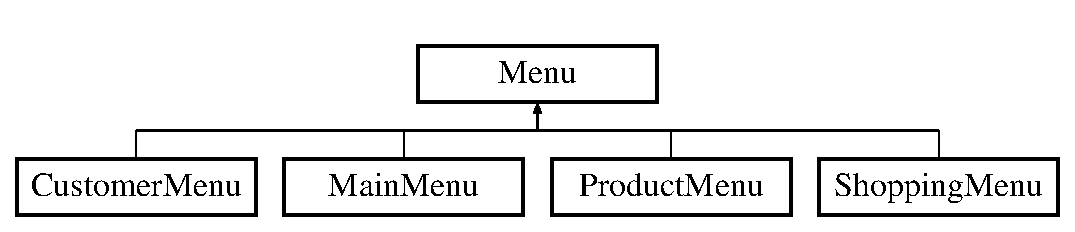
\includegraphics[height=2.000000cm]{classMenu}
\end{center}
\end{figure}
\subsection*{Public Member Functions}
\begin{DoxyCompactItemize}
\item 
\mbox{\Hypertarget{classMenu_a3377fd5036a2f8f93eee473afd570185}\label{classMenu_a3377fd5036a2f8f93eee473afd570185}} 
\hyperlink{classMenu_a3377fd5036a2f8f93eee473afd570185}{Menu} (string title)
\begin{DoxyCompactList}\small\item\em Constructor with one arguments. \end{DoxyCompactList}\item 
\hyperlink{classMenu_a28dcf937389ad94a178caef7b28a11a8}{Menu} (string, string $\ast$, int)
\begin{DoxyCompactList}\small\item\em Constructor with three arguments. \end{DoxyCompactList}\item 
\hyperlink{classMenu_a831387f51358cfb88cd018e1777bc980}{$\sim$\+Menu} ()
\begin{DoxyCompactList}\small\item\em Destructor. \end{DoxyCompactList}\item 
void \hyperlink{classMenu_a2be45a29dd0fa643d5fc118350bce944}{add} (string $\ast$, int)
\begin{DoxyCompactList}\small\item\em Adds submenu. \end{DoxyCompactList}\item 
void \hyperlink{classMenu_a5423c0d700c20bf8bdd0fb1dbf0c0f6f}{add} (string)
\begin{DoxyCompactList}\small\item\em Adds submenu. \end{DoxyCompactList}\item 
int \hyperlink{classMenu_a346009151f57e18ffe0fa5a9dd89b1d6}{show} ()
\begin{DoxyCompactList}\small\item\em Shows submenus. \end{DoxyCompactList}\item 
\mbox{\Hypertarget{classMenu_ae9d7af36b1a380e5e4b03ddbef9ceeca}\label{classMenu_ae9d7af36b1a380e5e4b03ddbef9ceeca}} 
virtual void \hyperlink{classMenu_ae9d7af36b1a380e5e4b03ddbef9ceeca}{menu\+Switch} (int)=0
\begin{DoxyCompactList}\small\item\em Switchs to menu. \end{DoxyCompactList}\end{DoxyCompactItemize}
\subsection*{Protected Attributes}
\begin{DoxyCompactItemize}
\item 
\mbox{\Hypertarget{classMenu_a0edddfda0319fc24d00ca6ed610ea59b}\label{classMenu_a0edddfda0319fc24d00ca6ed610ea59b}} 
string {\bfseries title}
\item 
\mbox{\Hypertarget{classMenu_acfa8e5e2ebe7e383c2ea38c74be347c0}\label{classMenu_acfa8e5e2ebe7e383c2ea38c74be347c0}} 
vector$<$ string $>$ {\bfseries sub\+Menus}
\end{DoxyCompactItemize}


\subsection{Detailed Description}
\hyperlink{classMenu}{Menu} class. 

\subsection{Constructor \& Destructor Documentation}
\mbox{\Hypertarget{classMenu_a28dcf937389ad94a178caef7b28a11a8}\label{classMenu_a28dcf937389ad94a178caef7b28a11a8}} 
\index{Menu@{Menu}!Menu@{Menu}}
\index{Menu@{Menu}!Menu@{Menu}}
\subsubsection{\texorpdfstring{Menu()}{Menu()}}
{\footnotesize\ttfamily Menu\+::\+Menu (\begin{DoxyParamCaption}\item[{string}]{,  }\item[{string $\ast$}]{submenuarray,  }\item[{int}]{size }\end{DoxyParamCaption})}



Constructor with three arguments. 


\begin{DoxyParams}{Parameters}
{\em s} & a string argument. \\
\hline
{\em submenuarray} & a string argument. \\
\hline
{\em size} & an integer argument. \\
\hline
\end{DoxyParams}
\mbox{\Hypertarget{classMenu_a831387f51358cfb88cd018e1777bc980}\label{classMenu_a831387f51358cfb88cd018e1777bc980}} 
\index{Menu@{Menu}!````~Menu@{$\sim$\+Menu}}
\index{````~Menu@{$\sim$\+Menu}!Menu@{Menu}}
\subsubsection{\texorpdfstring{$\sim$\+Menu()}{~Menu()}}
{\footnotesize\ttfamily Menu\+::$\sim$\+Menu (\begin{DoxyParamCaption}{ }\end{DoxyParamCaption})}



Destructor. 

\hyperlink{classMenu}{Menu} class. 

\subsection{Member Function Documentation}
\mbox{\Hypertarget{classMenu_a2be45a29dd0fa643d5fc118350bce944}\label{classMenu_a2be45a29dd0fa643d5fc118350bce944}} 
\index{Menu@{Menu}!add@{add}}
\index{add@{add}!Menu@{Menu}}
\subsubsection{\texorpdfstring{add()}{add()}\hspace{0.1cm}{\footnotesize\ttfamily [1/2]}}
{\footnotesize\ttfamily void Menu\+::add (\begin{DoxyParamCaption}\item[{string $\ast$}]{submenuarray,  }\item[{int}]{size }\end{DoxyParamCaption})}



Adds submenu. 


\begin{DoxyParams}{Parameters}
{\em submenuarray} & a string argument. \\
\hline
\end{DoxyParams}
\mbox{\Hypertarget{classMenu_a5423c0d700c20bf8bdd0fb1dbf0c0f6f}\label{classMenu_a5423c0d700c20bf8bdd0fb1dbf0c0f6f}} 
\index{Menu@{Menu}!add@{add}}
\index{add@{add}!Menu@{Menu}}
\subsubsection{\texorpdfstring{add()}{add()}\hspace{0.1cm}{\footnotesize\ttfamily [2/2]}}
{\footnotesize\ttfamily void Menu\+::add (\begin{DoxyParamCaption}\item[{string}]{submenu }\end{DoxyParamCaption})}



Adds submenu. 


\begin{DoxyParams}{Parameters}
{\em submenu} & a string argument. \\
\hline
\end{DoxyParams}
\mbox{\Hypertarget{classMenu_a346009151f57e18ffe0fa5a9dd89b1d6}\label{classMenu_a346009151f57e18ffe0fa5a9dd89b1d6}} 
\index{Menu@{Menu}!show@{show}}
\index{show@{show}!Menu@{Menu}}
\subsubsection{\texorpdfstring{show()}{show()}}
{\footnotesize\ttfamily int Menu\+::show (\begin{DoxyParamCaption}{ }\end{DoxyParamCaption})}



Shows submenus. 

\begin{DoxyReturn}{Returns}
menu\+Input an integer argument. 
\end{DoxyReturn}


The documentation for this class was generated from the following files\+:\begin{DoxyCompactItemize}
\item 
Menu.\+h\item 
Menu.\+cpp\end{DoxyCompactItemize}

\hypertarget{classMusicCD}{}\section{Music\+CD Class Reference}
\label{classMusicCD}\index{Music\+CD@{Music\+CD}}


\hyperlink{classMusicCD}{Music\+CD} class inherits from product class.  




{\ttfamily \#include $<$Music\+C\+D.\+h$>$}

Inheritance diagram for Music\+CD\+:\begin{figure}[H]
\begin{center}
\leavevmode
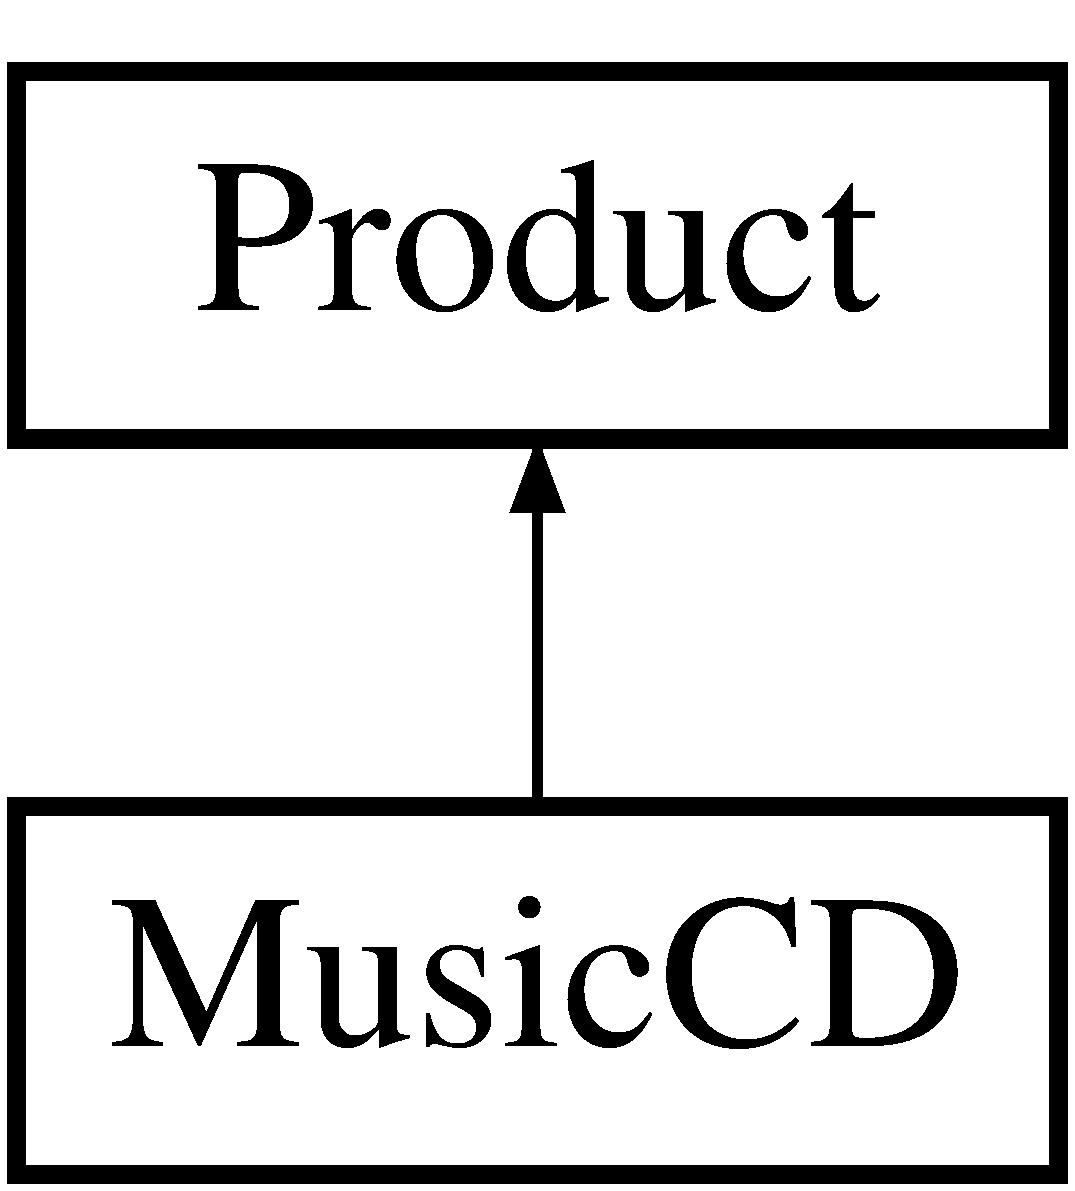
\includegraphics[height=2.000000cm]{classMusicCD}
\end{center}
\end{figure}
\subsection*{Public Member Functions}
\begin{DoxyCompactItemize}
\item 
\hyperlink{classMusicCD_a334b0680f6901e6d4f34791aecf075fd}{Music\+CD} (int, string, double, string, string)
\begin{DoxyCompactList}\small\item\em Constructor with five arguments. \end{DoxyCompactList}\item 
\hyperlink{classMusicCD_aecdf5af2b88efcd0f3e0d5722f0316d3}{Music\+CD} (int, string, double)
\begin{DoxyCompactList}\small\item\em Constructor with three arguments. \end{DoxyCompactList}\item 
\mbox{\Hypertarget{classMusicCD_ab484d97087a7eb43716b2f96da6b44d1}\label{classMusicCD_ab484d97087a7eb43716b2f96da6b44d1}} 
virtual \hyperlink{classMusicCD_ab484d97087a7eb43716b2f96da6b44d1}{$\sim$\+Music\+CD} ()
\begin{DoxyCompactList}\small\item\em Destructor. \end{DoxyCompactList}\item 
\mbox{\Hypertarget{classMusicCD_a86f5945b7f17a544ccb286e38058b550}\label{classMusicCD_a86f5945b7f17a544ccb286e38058b550}} 
void {\bfseries print\+Properties} ()
\item 
string \hyperlink{classMusicCD_afb4af62b3ba9ba78ee348a94c0fb2a21}{get\+Singer} () const
\begin{DoxyCompactList}\small\item\em Gets singer. \end{DoxyCompactList}\item 
void \hyperlink{classMusicCD_a1a425710dfc010eb5f2bbde63d53f89d}{set\+Singer} (string)
\begin{DoxyCompactList}\small\item\em Sets singer. \end{DoxyCompactList}\item 
string \hyperlink{classMusicCD_aa60af83051f83827e56b7ebaf3d459d2}{get\+Type} () const
\begin{DoxyCompactList}\small\item\em Gets type. \end{DoxyCompactList}\item 
void \hyperlink{classMusicCD_a1b1ea75abec58c4154dee842f9833995}{set\+Type} (string)
\begin{DoxyCompactList}\small\item\em Sets type. \end{DoxyCompactList}\end{DoxyCompactItemize}


\subsection{Detailed Description}
\hyperlink{classMusicCD}{Music\+CD} class inherits from product class. 

\subsection{Constructor \& Destructor Documentation}
\mbox{\Hypertarget{classMusicCD_a334b0680f6901e6d4f34791aecf075fd}\label{classMusicCD_a334b0680f6901e6d4f34791aecf075fd}} 
\index{Music\+CD@{Music\+CD}!Music\+CD@{Music\+CD}}
\index{Music\+CD@{Music\+CD}!Music\+CD@{Music\+CD}}
\subsubsection{\texorpdfstring{Music\+C\+D()}{MusicCD()}\hspace{0.1cm}{\footnotesize\ttfamily [1/2]}}
{\footnotesize\ttfamily Music\+C\+D\+::\+Music\+CD (\begin{DoxyParamCaption}\item[{int}]{id,  }\item[{string}]{name,  }\item[{double}]{price,  }\item[{string}]{singer,  }\item[{string}]{type }\end{DoxyParamCaption})}



Constructor with five arguments. 


\begin{DoxyParams}{Parameters}
{\em name} & a string argument. \\
\hline
{\em singer} & a string argument. \\
\hline
{\em type} & a string argument. \\
\hline
{\em id} & a integer argument. \\
\hline
{\em price} & a double argument. \\
\hline
\end{DoxyParams}
\mbox{\Hypertarget{classMusicCD_aecdf5af2b88efcd0f3e0d5722f0316d3}\label{classMusicCD_aecdf5af2b88efcd0f3e0d5722f0316d3}} 
\index{Music\+CD@{Music\+CD}!Music\+CD@{Music\+CD}}
\index{Music\+CD@{Music\+CD}!Music\+CD@{Music\+CD}}
\subsubsection{\texorpdfstring{Music\+C\+D()}{MusicCD()}\hspace{0.1cm}{\footnotesize\ttfamily [2/2]}}
{\footnotesize\ttfamily Music\+C\+D\+::\+Music\+CD (\begin{DoxyParamCaption}\item[{int}]{id,  }\item[{string}]{name,  }\item[{double}]{price }\end{DoxyParamCaption})}



Constructor with three arguments. 


\begin{DoxyParams}{Parameters}
{\em name} & a string argument. \\
\hline
{\em id} & a integer argument. \\
\hline
{\em price} & a double argument. \\
\hline
\end{DoxyParams}


\subsection{Member Function Documentation}
\mbox{\Hypertarget{classMusicCD_afb4af62b3ba9ba78ee348a94c0fb2a21}\label{classMusicCD_afb4af62b3ba9ba78ee348a94c0fb2a21}} 
\index{Music\+CD@{Music\+CD}!get\+Singer@{get\+Singer}}
\index{get\+Singer@{get\+Singer}!Music\+CD@{Music\+CD}}
\subsubsection{\texorpdfstring{get\+Singer()}{getSinger()}}
{\footnotesize\ttfamily string Music\+C\+D\+::get\+Singer (\begin{DoxyParamCaption}{ }\end{DoxyParamCaption}) const}



Gets singer. 

\hyperlink{classMusicCD}{Music\+CD} class.

\begin{DoxyReturn}{Returns}
singer a string argument. 
\end{DoxyReturn}
\mbox{\Hypertarget{classMusicCD_aa60af83051f83827e56b7ebaf3d459d2}\label{classMusicCD_aa60af83051f83827e56b7ebaf3d459d2}} 
\index{Music\+CD@{Music\+CD}!get\+Type@{get\+Type}}
\index{get\+Type@{get\+Type}!Music\+CD@{Music\+CD}}
\subsubsection{\texorpdfstring{get\+Type()}{getType()}}
{\footnotesize\ttfamily string Music\+C\+D\+::get\+Type (\begin{DoxyParamCaption}{ }\end{DoxyParamCaption}) const}



Gets type. 

\begin{DoxyReturn}{Returns}
type a string argument. 
\end{DoxyReturn}
\mbox{\Hypertarget{classMusicCD_a1a425710dfc010eb5f2bbde63d53f89d}\label{classMusicCD_a1a425710dfc010eb5f2bbde63d53f89d}} 
\index{Music\+CD@{Music\+CD}!set\+Singer@{set\+Singer}}
\index{set\+Singer@{set\+Singer}!Music\+CD@{Music\+CD}}
\subsubsection{\texorpdfstring{set\+Singer()}{setSinger()}}
{\footnotesize\ttfamily void Music\+C\+D\+::set\+Singer (\begin{DoxyParamCaption}\item[{string}]{ }\end{DoxyParamCaption})}



Sets singer. 


\begin{DoxyParams}{Parameters}
{\em singer} & a string argument. \\
\hline
\end{DoxyParams}
\mbox{\Hypertarget{classMusicCD_a1b1ea75abec58c4154dee842f9833995}\label{classMusicCD_a1b1ea75abec58c4154dee842f9833995}} 
\index{Music\+CD@{Music\+CD}!set\+Type@{set\+Type}}
\index{set\+Type@{set\+Type}!Music\+CD@{Music\+CD}}
\subsubsection{\texorpdfstring{set\+Type()}{setType()}}
{\footnotesize\ttfamily void Music\+C\+D\+::set\+Type (\begin{DoxyParamCaption}\item[{string}]{ }\end{DoxyParamCaption})}



Sets type. 


\begin{DoxyParams}{Parameters}
{\em type} & a string argument. \\
\hline
\end{DoxyParams}


The documentation for this class was generated from the following files\+:\begin{DoxyCompactItemize}
\item 
Music\+C\+D.\+h\item 
Music\+C\+D.\+cpp\end{DoxyCompactItemize}

\hypertarget{classPayment}{}\section{Payment Class Reference}
\label{classPayment}\index{Payment@{Payment}}


\hyperlink{classPayment}{Payment} class.  




{\ttfamily \#include $<$Payment.\+h$>$}

Inheritance diagram for Payment\+:\begin{figure}[H]
\begin{center}
\leavevmode
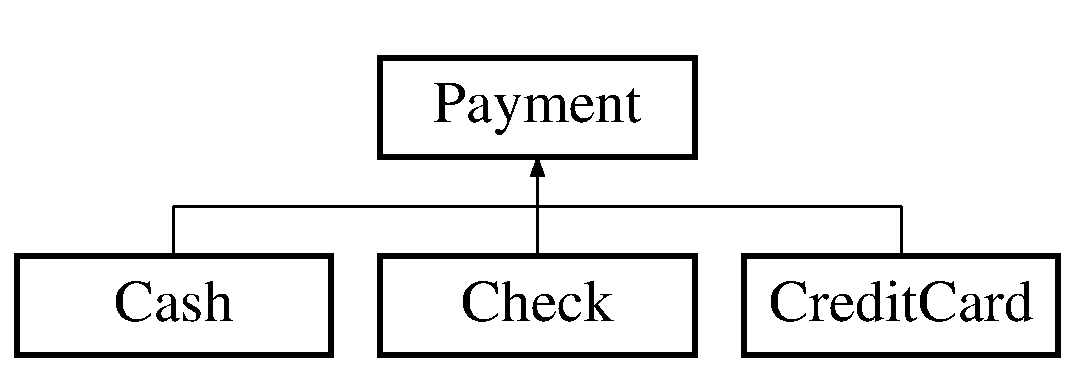
\includegraphics[height=2.000000cm]{classPayment}
\end{center}
\end{figure}
\subsection*{Public Member Functions}
\begin{DoxyCompactItemize}
\item 
\hyperlink{classPayment_abe05f968db46b0211379eeee357ef58d}{Payment} (double)
\begin{DoxyCompactList}\small\item\em Constructor with one arguments. \end{DoxyCompactList}\item 
\mbox{\Hypertarget{classPayment_acc52d8f5b5b333f8acd89611f4926082}\label{classPayment_acc52d8f5b5b333f8acd89611f4926082}} 
virtual \hyperlink{classPayment_acc52d8f5b5b333f8acd89611f4926082}{$\sim$\+Payment} ()
\begin{DoxyCompactList}\small\item\em Destructor. \end{DoxyCompactList}\item 
double \hyperlink{classPayment_a589cf7d06f7365d5505948bdef033828}{get\+Amount} () const
\begin{DoxyCompactList}\small\item\em Gets amount. \end{DoxyCompactList}\item 
void \hyperlink{classPayment_ae967c922e523959e20933da449e5d0fd}{set\+Amount} (double)
\begin{DoxyCompactList}\small\item\em Sets amount. \end{DoxyCompactList}\item 
\mbox{\Hypertarget{classPayment_afc011ab4bc8dee83b184bdc056d4c2a9}\label{classPayment_afc011ab4bc8dee83b184bdc056d4c2a9}} 
virtual void \hyperlink{classPayment_afc011ab4bc8dee83b184bdc056d4c2a9}{perform\+Payment} ()=0
\begin{DoxyCompactList}\small\item\em About perform\+Payment. \end{DoxyCompactList}\item 
\mbox{\Hypertarget{classPayment_ae3be1f239771fbe95b173a82e4b49543}\label{classPayment_ae3be1f239771fbe95b173a82e4b49543}} 
virtual string \hyperlink{classPayment_ae3be1f239771fbe95b173a82e4b49543}{payment\+Info} ()=0
\begin{DoxyCompactList}\small\item\em About payment informations. \end{DoxyCompactList}\end{DoxyCompactItemize}


\subsection{Detailed Description}
\hyperlink{classPayment}{Payment} class. 

\subsection{Constructor \& Destructor Documentation}
\mbox{\Hypertarget{classPayment_abe05f968db46b0211379eeee357ef58d}\label{classPayment_abe05f968db46b0211379eeee357ef58d}} 
\index{Payment@{Payment}!Payment@{Payment}}
\index{Payment@{Payment}!Payment@{Payment}}
\subsubsection{\texorpdfstring{Payment()}{Payment()}}
{\footnotesize\ttfamily Payment\+::\+Payment (\begin{DoxyParamCaption}\item[{double}]{amount }\end{DoxyParamCaption})}



Constructor with one arguments. 


\begin{DoxyParams}{Parameters}
{\em amount} & a double argument. \\
\hline
\end{DoxyParams}


\subsection{Member Function Documentation}
\mbox{\Hypertarget{classPayment_a589cf7d06f7365d5505948bdef033828}\label{classPayment_a589cf7d06f7365d5505948bdef033828}} 
\index{Payment@{Payment}!get\+Amount@{get\+Amount}}
\index{get\+Amount@{get\+Amount}!Payment@{Payment}}
\subsubsection{\texorpdfstring{get\+Amount()}{getAmount()}}
{\footnotesize\ttfamily double Payment\+::get\+Amount (\begin{DoxyParamCaption}{ }\end{DoxyParamCaption}) const}



Gets amount. 

\hyperlink{classPayment}{Payment} class.

\begin{DoxyReturn}{Returns}
amount a double argument. 
\end{DoxyReturn}
\mbox{\Hypertarget{classPayment_ae967c922e523959e20933da449e5d0fd}\label{classPayment_ae967c922e523959e20933da449e5d0fd}} 
\index{Payment@{Payment}!set\+Amount@{set\+Amount}}
\index{set\+Amount@{set\+Amount}!Payment@{Payment}}
\subsubsection{\texorpdfstring{set\+Amount()}{setAmount()}}
{\footnotesize\ttfamily void Payment\+::set\+Amount (\begin{DoxyParamCaption}\item[{double}]{amount }\end{DoxyParamCaption})}



Sets amount. 

amount a double argument. 

The documentation for this class was generated from the following files\+:\begin{DoxyCompactItemize}
\item 
Payment.\+h\item 
Payment.\+cpp\end{DoxyCompactItemize}

\hypertarget{classProduct}{}\section{Product Class Reference}
\label{classProduct}\index{Product@{Product}}


\hyperlink{classProduct}{Product} class.  




{\ttfamily \#include $<$Product.\+h$>$}

Inheritance diagram for Product\+:\begin{figure}[H]
\begin{center}
\leavevmode
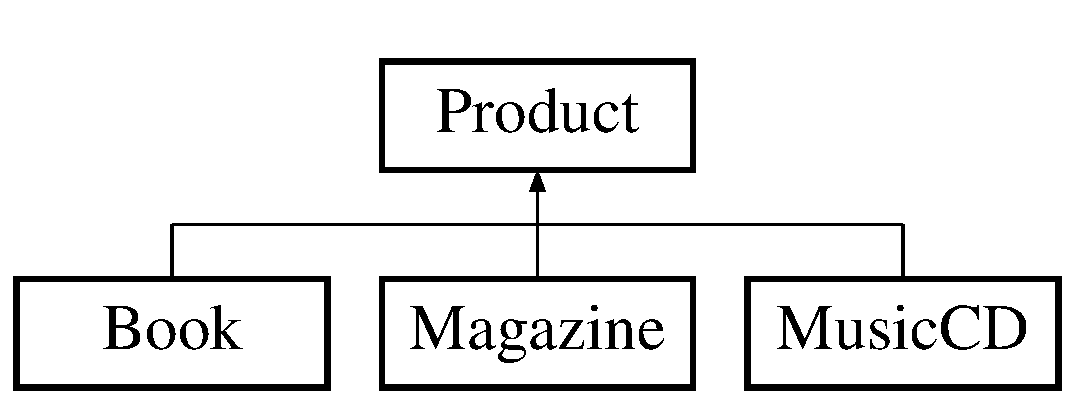
\includegraphics[height=2.000000cm]{classProduct}
\end{center}
\end{figure}
\subsection*{Public Member Functions}
\begin{DoxyCompactItemize}
\item 
\hyperlink{classProduct_aa7705364efa0a211575a00b5a6b8537c}{Product} (int, string, double)
\begin{DoxyCompactList}\small\item\em Constructor with three arguments. \end{DoxyCompactList}\item 
\mbox{\Hypertarget{classProduct_abe0afd3bea96d979185ec2cfdf681e6f}\label{classProduct_abe0afd3bea96d979185ec2cfdf681e6f}} 
\hyperlink{classProduct_abe0afd3bea96d979185ec2cfdf681e6f}{$\sim$\+Product} ()
\begin{DoxyCompactList}\small\item\em Destructor. \end{DoxyCompactList}\item 
int \hyperlink{classProduct_a6cca56300caa309ce1f256a75b7afb32}{get\+Id} () const
\begin{DoxyCompactList}\small\item\em Gets Id. \end{DoxyCompactList}\item 
void \hyperlink{classProduct_afeb389b5d13ac1e68bbdafe41c898689}{set\+Id} (int)
\begin{DoxyCompactList}\small\item\em Sets Id. \end{DoxyCompactList}\item 
string \hyperlink{classProduct_add69128805228e23dcc6619b0a167a08}{get\+Name} () const
\begin{DoxyCompactList}\small\item\em Gets name. \end{DoxyCompactList}\item 
void \hyperlink{classProduct_ae5aa54c86d99f87b2b6bca4aa1a0479f}{set\+Name} (string)
\begin{DoxyCompactList}\small\item\em Sets name. \end{DoxyCompactList}\item 
double \hyperlink{classProduct_a3be25f647260d61df6063ef706261c7f}{get\+Price} () const
\begin{DoxyCompactList}\small\item\em Gets price. \end{DoxyCompactList}\item 
void \hyperlink{classProduct_aacd8e249939d497c95881ae859280d48}{set\+Price} (double)
\begin{DoxyCompactList}\small\item\em Sets price. \end{DoxyCompactList}\item 
\mbox{\Hypertarget{classProduct_a2258435eb75f901b13f44f83da4927d8}\label{classProduct_a2258435eb75f901b13f44f83da4927d8}} 
virtual void {\bfseries print\+Properties} ()=0
\end{DoxyCompactItemize}


\subsection{Detailed Description}
\hyperlink{classProduct}{Product} class. 

\subsection{Constructor \& Destructor Documentation}
\mbox{\Hypertarget{classProduct_aa7705364efa0a211575a00b5a6b8537c}\label{classProduct_aa7705364efa0a211575a00b5a6b8537c}} 
\index{Product@{Product}!Product@{Product}}
\index{Product@{Product}!Product@{Product}}
\subsubsection{\texorpdfstring{Product()}{Product()}}
{\footnotesize\ttfamily Product\+::\+Product (\begin{DoxyParamCaption}\item[{int}]{id,  }\item[{string}]{name,  }\item[{double}]{price }\end{DoxyParamCaption})}



Constructor with three arguments. 


\begin{DoxyParams}{Parameters}
{\em id} & an integer argument. \\
\hline
{\em name} & a string argument. \\
\hline
{\em price} & a double argument. \\
\hline
\end{DoxyParams}


\subsection{Member Function Documentation}
\mbox{\Hypertarget{classProduct_a6cca56300caa309ce1f256a75b7afb32}\label{classProduct_a6cca56300caa309ce1f256a75b7afb32}} 
\index{Product@{Product}!get\+Id@{get\+Id}}
\index{get\+Id@{get\+Id}!Product@{Product}}
\subsubsection{\texorpdfstring{get\+Id()}{getId()}}
{\footnotesize\ttfamily int Product\+::get\+Id (\begin{DoxyParamCaption}{ }\end{DoxyParamCaption}) const}



Gets Id. 

product class.

\begin{DoxyReturn}{Returns}
id an integer argument. 
\end{DoxyReturn}
\mbox{\Hypertarget{classProduct_add69128805228e23dcc6619b0a167a08}\label{classProduct_add69128805228e23dcc6619b0a167a08}} 
\index{Product@{Product}!get\+Name@{get\+Name}}
\index{get\+Name@{get\+Name}!Product@{Product}}
\subsubsection{\texorpdfstring{get\+Name()}{getName()}}
{\footnotesize\ttfamily string Product\+::get\+Name (\begin{DoxyParamCaption}{ }\end{DoxyParamCaption}) const}



Gets name. 

\begin{DoxyReturn}{Returns}
name a string argument. 
\end{DoxyReturn}
\mbox{\Hypertarget{classProduct_a3be25f647260d61df6063ef706261c7f}\label{classProduct_a3be25f647260d61df6063ef706261c7f}} 
\index{Product@{Product}!get\+Price@{get\+Price}}
\index{get\+Price@{get\+Price}!Product@{Product}}
\subsubsection{\texorpdfstring{get\+Price()}{getPrice()}}
{\footnotesize\ttfamily double Product\+::get\+Price (\begin{DoxyParamCaption}{ }\end{DoxyParamCaption}) const}



Gets price. 

\begin{DoxyReturn}{Returns}
price a double argument. 
\end{DoxyReturn}
\mbox{\Hypertarget{classProduct_afeb389b5d13ac1e68bbdafe41c898689}\label{classProduct_afeb389b5d13ac1e68bbdafe41c898689}} 
\index{Product@{Product}!set\+Id@{set\+Id}}
\index{set\+Id@{set\+Id}!Product@{Product}}
\subsubsection{\texorpdfstring{set\+Id()}{setId()}}
{\footnotesize\ttfamily void Product\+::set\+Id (\begin{DoxyParamCaption}\item[{int}]{id }\end{DoxyParamCaption})}



Sets Id. 


\begin{DoxyParams}{Parameters}
{\em id} & an integer argument. \\
\hline
\end{DoxyParams}
\mbox{\Hypertarget{classProduct_ae5aa54c86d99f87b2b6bca4aa1a0479f}\label{classProduct_ae5aa54c86d99f87b2b6bca4aa1a0479f}} 
\index{Product@{Product}!set\+Name@{set\+Name}}
\index{set\+Name@{set\+Name}!Product@{Product}}
\subsubsection{\texorpdfstring{set\+Name()}{setName()}}
{\footnotesize\ttfamily void Product\+::set\+Name (\begin{DoxyParamCaption}\item[{string}]{name }\end{DoxyParamCaption})}



Sets name. 


\begin{DoxyParams}{Parameters}
{\em name} & a string argument. \\
\hline
\end{DoxyParams}
\mbox{\Hypertarget{classProduct_aacd8e249939d497c95881ae859280d48}\label{classProduct_aacd8e249939d497c95881ae859280d48}} 
\index{Product@{Product}!set\+Price@{set\+Price}}
\index{set\+Price@{set\+Price}!Product@{Product}}
\subsubsection{\texorpdfstring{set\+Price()}{setPrice()}}
{\footnotesize\ttfamily void Product\+::set\+Price (\begin{DoxyParamCaption}\item[{double}]{price }\end{DoxyParamCaption})}



Sets price. 


\begin{DoxyParams}{Parameters}
{\em price} & a double argument. \\
\hline
\end{DoxyParams}


The documentation for this class was generated from the following files\+:\begin{DoxyCompactItemize}
\item 
Product.\+h\item 
Product.\+cpp\end{DoxyCompactItemize}

\hypertarget{classProductMenu}{}\section{Product\+Menu Class Reference}
\label{classProductMenu}\index{Product\+Menu@{Product\+Menu}}
Inheritance diagram for Product\+Menu\+:\begin{figure}[H]
\begin{center}
\leavevmode
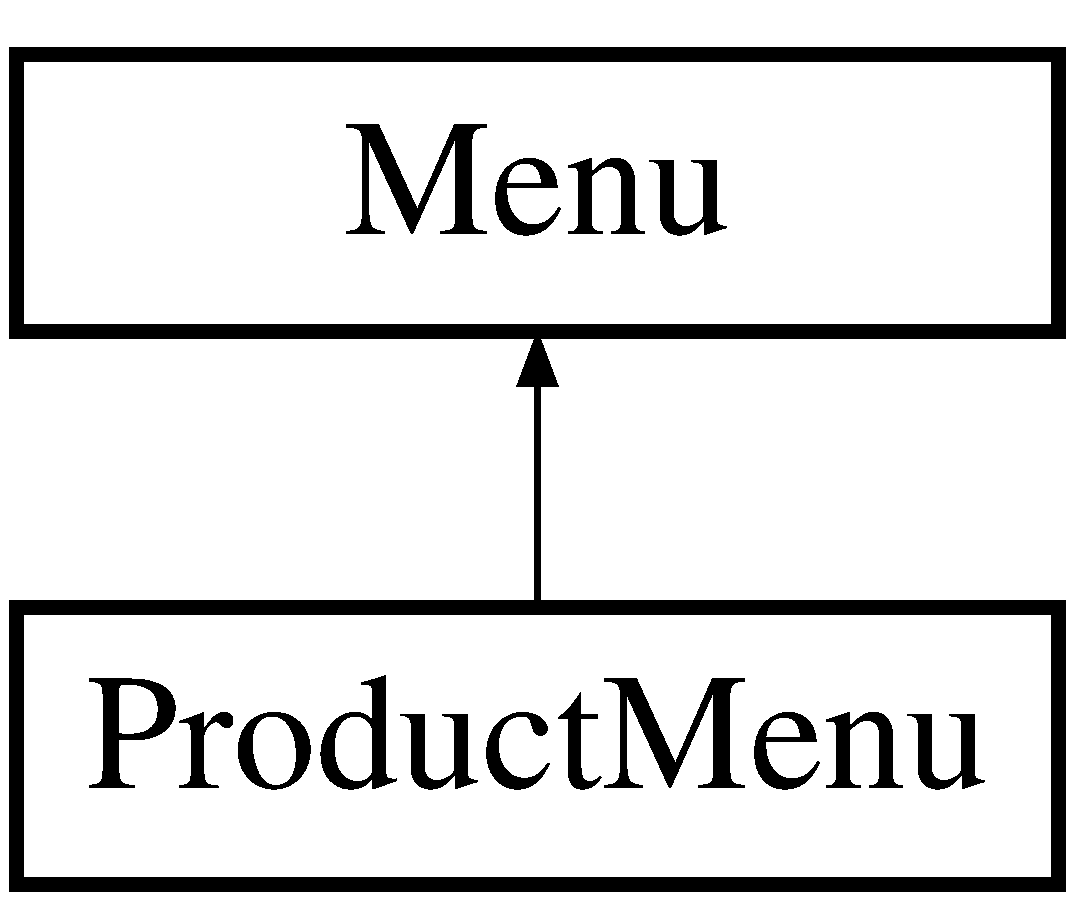
\includegraphics[height=2.000000cm]{classProductMenu}
\end{center}
\end{figure}
\subsection*{Public Member Functions}
\begin{DoxyCompactItemize}
\item 
\mbox{\Hypertarget{classProductMenu_a82b4acc7ccba704e2a54d3259b361230}\label{classProductMenu_a82b4acc7ccba704e2a54d3259b361230}} 
{\bfseries Product\+Menu} (string title, string $\ast$subs, int size, vector$<$ \hyperlink{classProduct}{Product} $\ast$$>$ p\+List)
\item 
\mbox{\Hypertarget{classProductMenu_a0f8a319dae390c983d728219cf845aef}\label{classProductMenu_a0f8a319dae390c983d728219cf845aef}} 
const vector$<$ \hyperlink{classProduct}{Product} $\ast$ $>$ \& {\bfseries get\+Product\+List} () const
\item 
\mbox{\Hypertarget{classProductMenu_a4aaea1df5f79ec3d744c1810a6ab03e2}\label{classProductMenu_a4aaea1df5f79ec3d744c1810a6ab03e2}} 
void {\bfseries set\+Product\+List} (const vector$<$ \hyperlink{classProduct}{Product} $\ast$$>$ \&product\+List)
\item 
\mbox{\Hypertarget{classProductMenu_a24a18c11760a828b7b7de4acc22bcce5}\label{classProductMenu_a24a18c11760a828b7b7de4acc22bcce5}} 
void \hyperlink{classProductMenu_a24a18c11760a828b7b7de4acc22bcce5}{menu\+Switch} (int)
\begin{DoxyCompactList}\small\item\em Switchs to menu. \end{DoxyCompactList}\end{DoxyCompactItemize}
\subsection*{Additional Inherited Members}


The documentation for this class was generated from the following files\+:\begin{DoxyCompactItemize}
\item 
Product\+Menu.\+h\item 
Product\+Menu.\+cpp\end{DoxyCompactItemize}

\hypertarget{classProductToPurchase}{}\section{Product\+To\+Purchase Class Reference}
\label{classProductToPurchase}\index{Product\+To\+Purchase@{Product\+To\+Purchase}}
\subsection*{Public Member Functions}
\begin{DoxyCompactItemize}
\item 
\mbox{\Hypertarget{classProductToPurchase_a65d9a7db4ea2986621bb4cf7fa9dd35f}\label{classProductToPurchase_a65d9a7db4ea2986621bb4cf7fa9dd35f}} 
{\bfseries Product\+To\+Purchase} (\hyperlink{classProduct}{Product} $\ast$, int=1)
\item 
\mbox{\Hypertarget{classProductToPurchase_a6eaebabfae95c423101ff08ac45d5a80}\label{classProductToPurchase_a6eaebabfae95c423101ff08ac45d5a80}} 
\hyperlink{classProduct}{Product} $\ast$ {\bfseries get\+Product} () const
\item 
\mbox{\Hypertarget{classProductToPurchase_abb61c6a0bf69664e220c2db208085267}\label{classProductToPurchase_abb61c6a0bf69664e220c2db208085267}} 
void {\bfseries set\+Product} (\hyperlink{classProduct}{Product} $\ast$)
\item 
\mbox{\Hypertarget{classProductToPurchase_a014993f945537561c6161914e9f981d4}\label{classProductToPurchase_a014993f945537561c6161914e9f981d4}} 
int {\bfseries get\+Quantity} () const
\item 
\mbox{\Hypertarget{classProductToPurchase_aa7dd27c6260de99906366f0a89a73439}\label{classProductToPurchase_aa7dd27c6260de99906366f0a89a73439}} 
void {\bfseries set\+Quantity} (int \+\_\+quantity)
\end{DoxyCompactItemize}


The documentation for this class was generated from the following files\+:\begin{DoxyCompactItemize}
\item 
Product\+To\+Purchase.\+h\item 
Product\+To\+Purchase.\+cpp\end{DoxyCompactItemize}

\hypertarget{classShoppingCart}{}\section{Shopping\+Cart Class Reference}
\label{classShoppingCart}\index{Shopping\+Cart@{Shopping\+Cart}}
\subsection*{Public Member Functions}
\begin{DoxyCompactItemize}
\item 
\mbox{\Hypertarget{classShoppingCart_af7a004471b1321cd7ee3b725be7bc7d7}\label{classShoppingCart_af7a004471b1321cd7ee3b725be7bc7d7}} 
{\bfseries Shopping\+Cart} (\hyperlink{classCustomer}{Customer} $\ast$)
\item 
\mbox{\Hypertarget{classShoppingCart_ad8b993ad16c3e9c741bba48ede71d37a}\label{classShoppingCart_ad8b993ad16c3e9c741bba48ede71d37a}} 
\hyperlink{classPayment}{Payment} $\ast$ {\bfseries get\+Payment\+Method} () const
\item 
\mbox{\Hypertarget{classShoppingCart_a1648a74b6b51553740a964d39732f62a}\label{classShoppingCart_a1648a74b6b51553740a964d39732f62a}} 
void {\bfseries set\+Payment\+Method} (\hyperlink{classPayment}{Payment} $\ast$)
\item 
\mbox{\Hypertarget{classShoppingCart_a21f92d071d2ce35e03175969ce82da79}\label{classShoppingCart_a21f92d071d2ce35e03175969ce82da79}} 
\hyperlink{classCustomer}{Customer} $\ast$ {\bfseries get\+Customer} () const
\item 
\mbox{\Hypertarget{classShoppingCart_afa31abf8f6244304419f4e6caf3b109c}\label{classShoppingCart_afa31abf8f6244304419f4e6caf3b109c}} 
void {\bfseries set\+Customer} (\hyperlink{classCustomer}{Customer} $\ast$)
\item 
\mbox{\Hypertarget{classShoppingCart_a2ed167d69492c61daf08754b4e3f99cf}\label{classShoppingCart_a2ed167d69492c61daf08754b4e3f99cf}} 
void {\bfseries set\+Bonus\+Used} ()
\item 
\mbox{\Hypertarget{classShoppingCart_afcab6367adfc0be9e37dd037a43b4ce2}\label{classShoppingCart_afcab6367adfc0be9e37dd037a43b4ce2}} 
void {\bfseries add\+Product} (\hyperlink{classProduct}{Product} $\ast$, int)
\item 
\mbox{\Hypertarget{classShoppingCart_ad82371a6788905b99e6a03e3cd359242}\label{classShoppingCart_ad82371a6788905b99e6a03e3cd359242}} 
void {\bfseries remove\+Product} (\hyperlink{classProduct}{Product} $\ast$)
\item 
\mbox{\Hypertarget{classShoppingCart_af02e91c37822093ea7d8a2d63e8601a4}\label{classShoppingCart_af02e91c37822093ea7d8a2d63e8601a4}} 
void {\bfseries place\+Order} ()
\item 
\mbox{\Hypertarget{classShoppingCart_a5c0c28d996ac9eba943ec6086065d958}\label{classShoppingCart_a5c0c28d996ac9eba943ec6086065d958}} 
void {\bfseries cancel\+Order} ()
\item 
\mbox{\Hypertarget{classShoppingCart_a157942fdeff8e09c48bbd745ab3cf1e4}\label{classShoppingCart_a157942fdeff8e09c48bbd745ab3cf1e4}} 
void {\bfseries print\+Products} ()
\item 
\mbox{\Hypertarget{classShoppingCart_a39a647d77d9dddbce4eb459f47d25dcc}\label{classShoppingCart_a39a647d77d9dddbce4eb459f47d25dcc}} 
string {\bfseries show\+Invoice} ()
\item 
\mbox{\Hypertarget{classShoppingCart_a13e1f55af8258d1beb8d343e1df7bf20}\label{classShoppingCart_a13e1f55af8258d1beb8d343e1df7bf20}} 
int {\bfseries get\+Product\+Count} ()
\item 
\mbox{\Hypertarget{classShoppingCart_ac09d762676e989a424e77f55299a0ee6}\label{classShoppingCart_ac09d762676e989a424e77f55299a0ee6}} 
double {\bfseries get\+Total\+Amount} ()
\end{DoxyCompactItemize}


The documentation for this class was generated from the following files\+:\begin{DoxyCompactItemize}
\item 
Shopping\+Cart.\+h\item 
Shopping\+Cart.\+cpp\end{DoxyCompactItemize}

\hypertarget{classShoppingMenu}{}\section{Shopping\+Menu Class Reference}
\label{classShoppingMenu}\index{Shopping\+Menu@{Shopping\+Menu}}
Inheritance diagram for Shopping\+Menu\+:\begin{figure}[H]
\begin{center}
\leavevmode
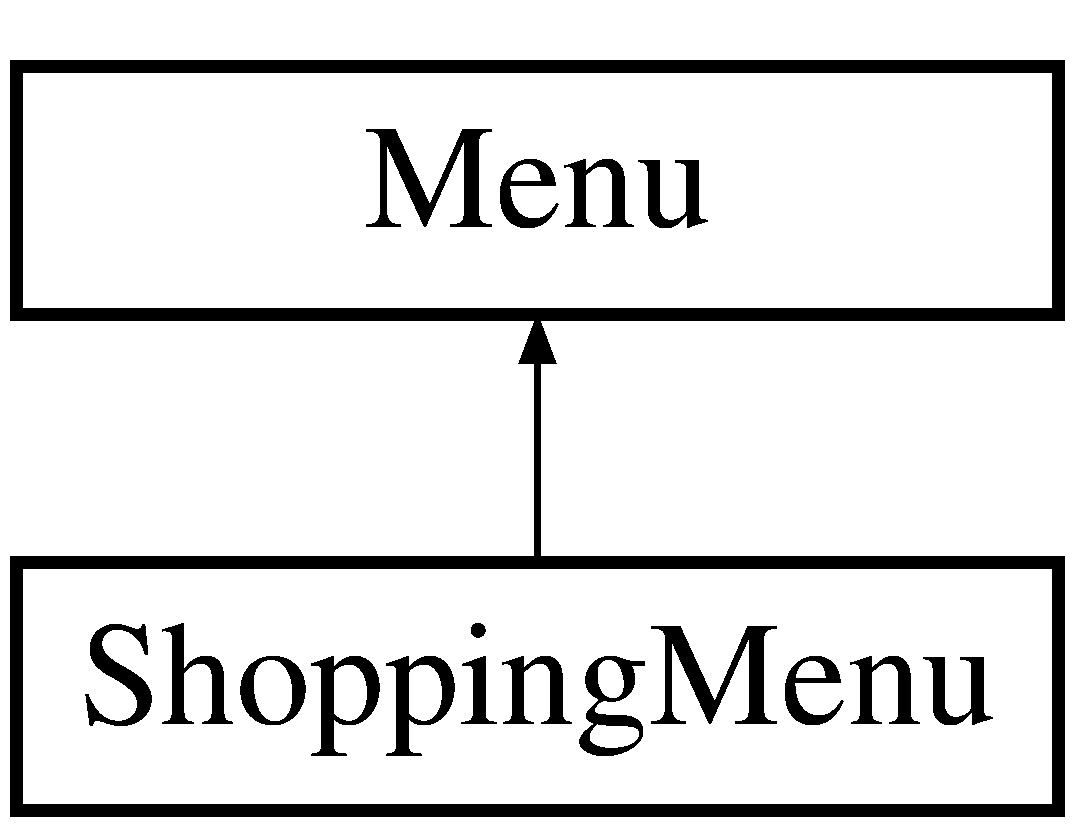
\includegraphics[height=2.000000cm]{classShoppingMenu}
\end{center}
\end{figure}
\subsection*{Public Member Functions}
\begin{DoxyCompactItemize}
\item 
\mbox{\Hypertarget{classShoppingMenu_ab2cac4b3c8eb0c57748f2dea30053048}\label{classShoppingMenu_ab2cac4b3c8eb0c57748f2dea30053048}} 
{\bfseries Shopping\+Menu} (string title, string $\ast$subs, int size, vector$<$ \hyperlink{classProduct}{Product} $\ast$$>$ p\+List, vector$<$ \hyperlink{classCustomer}{Customer} $>$ c\+List)
\item 
\mbox{\Hypertarget{classShoppingMenu_aaddca3b2c173197e0adfb230078ba7dc}\label{classShoppingMenu_aaddca3b2c173197e0adfb230078ba7dc}} 
const vector$<$ \hyperlink{classProduct}{Product} $\ast$ $>$ \& {\bfseries get\+Product\+List} () const
\item 
\mbox{\Hypertarget{classShoppingMenu_a19763d578bae9c29cad5ea091e5079a3}\label{classShoppingMenu_a19763d578bae9c29cad5ea091e5079a3}} 
void {\bfseries set\+Product\+List} (const vector$<$ \hyperlink{classProduct}{Product} $\ast$$>$ \&product\+List)
\item 
\mbox{\Hypertarget{classShoppingMenu_ae830bc8317c5c8e79bf25a82736dbdfb}\label{classShoppingMenu_ae830bc8317c5c8e79bf25a82736dbdfb}} 
const vector$<$ \hyperlink{classCustomer}{Customer} $>$ \& {\bfseries get\+Customer\+List} () const
\item 
\mbox{\Hypertarget{classShoppingMenu_a130e9b603e0307a6bc89e315b2ca968f}\label{classShoppingMenu_a130e9b603e0307a6bc89e315b2ca968f}} 
void {\bfseries set\+Customer\+List} (const vector$<$ \hyperlink{classCustomer}{Customer} $>$ \&customer\+List)
\item 
\mbox{\Hypertarget{classShoppingMenu_a2ae4f8b4fafbf970b454be146858c3d6}\label{classShoppingMenu_a2ae4f8b4fafbf970b454be146858c3d6}} 
void \hyperlink{classShoppingMenu_a2ae4f8b4fafbf970b454be146858c3d6}{menu\+Switch} (int)
\begin{DoxyCompactList}\small\item\em Switchs to menu. \end{DoxyCompactList}\end{DoxyCompactItemize}
\subsection*{Additional Inherited Members}


The documentation for this class was generated from the following files\+:\begin{DoxyCompactItemize}
\item 
Shopping\+Menu.\+h\item 
Shopping\+Menu.\+cpp\end{DoxyCompactItemize}

%--- End generated contents ---

% Index
\backmatter
\newpage
\phantomsection
\clearemptydoublepage
\addcontentsline{toc}{chapter}{Index}
\printindex

\end{document}
